\section{Empirical Evaluation}\label{sec:new:eval}
%\subsection{Empirical Evaluation}\label{sec:evaluation}
The empirical study aims at evaluating the performance of $\dpwcc$ when implemented in \acrshort{hs}. 
Our goal is to answer the following research questions: 

\begin{inparaenum}[\bf {\bf RQ}1\upshape)]
\label{res:question}
    \item Does $\dpwcc$ in \acrshort{hs} support the dynamic parallelization level that $\dpwcc$ requires?
    \item Is $\dpwcc$ in \acrshort{hs} competitive compared with default implementations on base libraries for the same problem?
    \item Does $\dpwcc$ in \acrshort{hs} handle memory efficiently?
\end{inparaenum}

We have conducted different kinds of experiments to test our assumptions and verify the correctness of the implementation.
First, we have performed an \emph{Implementation Analysis} in which we have selected some graphs from \acrfull{snap} \cite{stanford} and analyze how the implementation behaves under real-world graphs if it timeouts or not and if it is producing correct results in terms of the amount of \acrshort{wcc} that we know beforehand.
We have also tested the implementation doing a \emph{Benchmark Analysis} where we focus on two different types of benchmarks. On the one hand, using \texttt{criterion} library \cite{criterion}, we have evaluated a benchmark between our solution and \acrshort{wcc} algorithm implemented in \texttt{containers} \acrshort{hs} library\footnote{\url{https://hackage.haskell.org/package/containers}} using \mintinline{haskell}{Data.Graph}. On the other hand, we have compared if the results are being generated incrementally in both cases and how that is done during the pipeline execution time. This last analysis has been conducted using \texttt{diefpy} tool \cite{diefpaper,diefpy}.
Finally, we have executed a \textit{Performance Analysis} in which we have to gather profiling data from \acrfull{ghc} for one of the real-world graphs, to measure how the program performs regarding multithreading and memory allocation.

\paragraph{Running Architecture}
All the experiments have been executed in a $x86$ $64$ bits architecture with a \textit{$6$-Core Intel Core i7} processor of $2,2$ GHz which can emulate up to $12$ virtual cores. This processor has \emph{hyper-threading} enable. Regarding memory, the machine has $32 GB$ \emph{DDR4} of RAM, $256\ KB$ of L2 cache memory, and $9\ MB$ of L3 cache.

\paragraph{Haskell Setup}
Regarding specific libraries and compilations flags used on \acrshort{hs}, we have used \acrshort{ghc} version $8.10.4$. We have also used the following set of libraries: \mintinline{bash}{bytestring 0.10.12.0} \cite{bytestring}, \mintinline{bash}{containers 0.6.2.1} \cite{containers}, \mintinline{bash}{relude 1.0.0.1} \cite{relude} and \mintinline{bash}{unagi-chan 0.4.1.3} \cite{unagi}. The use of \texttt{relude} library is because we disabled \mintinline{haskell}{Prelude} from the project with the language extension \mintinline{haskell}{NoImplicitPrelude} \cite{extensions}. Regarding compilation flags (\acrshort{ghc} options) we have compiled our program with \mintinline{bash}{-threaded}, \mintinline{bash}{-O3}, \mintinline{bash}{-rtsopts}, \mintinline{bash}{-with-rtsopts=-N}. Since we have used \texttt{stack} version $2.5.1$ \cite{stack} as a building tool on top of \acrshort{ghc} the compilation command is \mintinline{bash}{stack build}\footnote{For more information about package.yaml or cabal file please check https://github.com/jproyo/upc-miri-tfm/tree/main/connected-comp}.

\paragraph{DataSets}\label{data:set}
For all the experiments, we have used the following networks taken from \acrshort{snap} \cite{stanford}. In this particular experiment setup, we have selected the following specific data sets that can be found here \cite{netenron, netastro, netwebgoogle}

\begin{table}[H]
  \centering
  \begin{tabular}{|p{0.25\linewidth}|r|r|r|r|r|}
   \hline
   \textbf{Network} & \textbf{Nodes} & \textbf{Edges} & \textbf{Diameter} & \textbf{\#\acrshort{wcc}} & \textbf{\#Nodes Largest WCC} \\
   \hline
   Enron Emails & 36692 & 183831 & 11 & 1065 & 33696 (0.918) \\
   \hline
   Astro Physics Collaboration Net & 18772 & 198110 & 14 & 290 & 17903 (0.954)\\
   \hline
   Google Web Graph & 875713 & 5105039 & 21 & 2746 & 855802 (0.977)\\
   \hline
  \end{tabular}
 \caption{DataSet of Graphs Selected}
 \label{table:4}
 \end{table}
 
 The criteria for selecting the networks have been followed the idea or testing the solution in more complex graphs, in which all of them are undirected but with different sizes concerning its number of nodes as we can see in  \autoref{table:4}. 
 %Smaller graphs have been tested as a part of the development cycle of the tool with automation testing libraries as it is described in \autoref{apx:1}.

\subsection{Experiments Definition}\label{sub:exp:def}
\paragraph{E1: Implementation Analysis}
In this experiment, we measure \acrshort{ghc} statistics running time enabling \mintinline{bash}{+RTS -s} flags. The metrics that we measure are \emph{MUT Time} which is the amount of time in seconds \acrshort{ghc} is running computations and \emph{GC Time} which is the number of seconds that \acrshort{ghc} is running garbage collector. \emph{Total execution time} is the sum of both in seconds. At the same time, we are going to check the correctness of the output counting the number of \acrshort{wcc} generated by the algorithm against the already known topology of it in \autoref{data:set}. The experiment's primary goal is to help answer the research question [RQ2].

\paragraph{E2: Benchmark Analysis}
In this experiment, we conduct two benchmark analysis over execution time comparing $DP_{WCC}$ in Haskell with \acrshort{hs} \texttt{containers} default implementation. In the first benchmark analysis, we use \texttt{criterion} \cite{criterion} tool in \acrshort{hs} which runs over four iterations of each of the algorithms to get a mean execution time in seconds and compare the results in a plot. In the second benchmark, we use \acrfull{dm} Tool \emph{diefpy} \cite{diefpy} in order to measure with the ability of \acrshort{dp} model to generate results incrementally \cite{diefpaper}. This is one of the strongest feature of \acrshort{dp} Paradigm since it allows process and generate results without no need of waiting for processing until the last element of the data source. This kind of aspect is essential not only for big data inputs where perhaps the requirements allow for processing until some point of the time having partial results but at the same time is important to process unbounded streams. The experiment's primary goal is to help answer the research question [RQ2] as well.

\paragraph{E3: Performance Analysis}
In this experiment, we measure internal parallelism in \acrshort{ghc} and memory usage during the execution of one of the example networks. The motivation of this is to verify empirically how $DP_{WCC}$ in Haskell is handling parallelization and memory usage. This experiment is conducted using two tools, \textit{ThreadScope} \cite{threadscope} for conducting multithreading analysis and \textit{eventlog2html} \cite{eventlog2html} to conduct memory usage analysis. Regarding multithreading analysis the metrics that we measure are the distribution of threads among processors over execution time which is how many processors are executing running threads over the whole execution; and the mean number of running threads per time slot which is calculated by zooming in $8$ time slots and taking the mean number of threads per processor to see if it is equally distributed among them. In regard to memory management, the metric that we measure is the amount of memory in $MB$ consumed per data type during the whole execution time. The experiment helps to answer the research questions [RQ1,RQ3].

\iffalse
\begin{table}[H]
  \centering
  \begin{tabular}{|l|p{0.16\linewidth}|p{0.2\linewidth}|p{0.2\linewidth}|p{0.2\linewidth}|l|}
   \hline
   \textbf{\#} & \textbf{Name} & \textbf{Goal} & \textbf{Motivation} & \textbf{How} & \textbf{RA} \\
   \hline
   \rule{0pt}{3ex}
   \multirow{2}{*}{\textbf{E1}} & Implementation Analysis & Measure GHC running time & Analyze execution time on Different Graph topologies & Enabling \mintinline{haskell}{+RTS -s} Flags & [Q2]  \\
   \cline{3-3} \cline{5-5} \rule{0pt}{3ex}
   & & Check correcteness of outputs &  & Redirect output and check amount of \acrshort{wcc} & \\
   \hline
    \rule{0pt}{3ex}
   \multirow{2}{*}{\textbf{E2}} & Benchmark Analysis & Measure execution time over $4$ iterations for each Graph from the selected DataSet, both for \acrshort{dp} and \texttt{containers} library & Compare execution time of both solutions & Use \emph{criterion} \cite{criterion} library  & [Q2] \\
   \cline{3-5} \rule{0pt}{3ex}
   & & Measure incremental generation of results, both for \acrshort{dp} and \texttt{containers} library & Compare diefficiency metrics & Use \emph{diefpy} \cite{diefpy} tool  & \\
   \hline
   \rule{0pt}{3ex}
   \textbf{E3} & Performance Analysis &Measure Internal Parallelism and Memory distribution of the solution & Verify empirically parallelization and memory behaviour of the program to asses the feasibility of the implementation & Use \emph{ThreadScope} \cite{threadscope} for Threading analysis and \emph{eventlog2html} \cite{eventlog2html} for memory analysis & [Q1,Q3]\\
   \hline
  \end{tabular}
 \caption{Experiments setup - Definition. RA (Research Answers)}
 \label{table:exp:1}
 \end{table}
\fi

\subsection{\textbf{Discussion of Observed Results}}\label{experiments}

\paragraph{Experiment: E1}\label{sub:sec:e1}
The following represents the execution for running these graphs on our \acrshort{dp} implementation.

\begin{table}[H]
  \centering
  \begin{tabular}{|l|r|r|r|r|}
   \hline
   \textbf{Network} & \textbf{Exec Param} & \textbf{MUT Time} & \textbf{GC Time} & \textbf{Total Time}\\
   \hline
   Enron Emails & \mintinline{bash}{+RTS -N4 -s} & 2.797s & 0.942s & 3.746s \\
   \hline
   Astro Physics Coll Net & \mintinline{bash}{+RTS -N4 -s} & 2.607s & 1.392s & 4.014s \\
   \hline
   Google Web Graph & \mintinline{bash}{+RTS -N8 -s} & 137.127s & 218.913s & \textbf{\textcolor{red}{356.058s}} \\
   \hline
  \end{tabular}
 \caption{Execution times}
 \label{table:5}
 \end{table}

It is important to point out that since the first two networks are smaller in the number of edges compared with \emph{web-Google}, executing those with $8$ cores as the \mintinline{bash}{-N} parameters indicates, does not affect the final speed-up since \acrshort{ghc} is not distributing threads on extra cores because it handles the load with $4$ cores only.

As we can see in \autoref{table:5}, we are obtaining remarkable execution times for the first two graphs and it seems not to be the case for \textit{web-Google}. Doing a deeper analysis on the topology of this last graph, we can see according to \autoref{table:4} that the number of \textit{Nodes in the largest \acrshort{wcc}} is the highest one. This means that there is a \acrshort{wcc} which contains $97.7\%$ of the nodes. Moreover, we can confirm that if we analyze even deeper how is the structure of that \acrshort{wcc} with the output of the algorithm, we can notice that the largest \acrshort{wcc} is the last one on being processed. Having that into consideration we can state that due to the nature of our algorithm which needs to wait for collecting all the vertices in the \mintinline{haskell}{actor2} filter stage 
%as it can be seen in \autoref{src:haskell:3}, 
it penalizes our execution time for that particular case. A more elaborated technique for implementing the actors is required to speed up execution. 

Regarding the correctness of the output, we have verified with the outputs that the number of connected components is the same as the metrics already gathered in \autoref{table:4}.

\paragraph{Experiment: E2}
\paragraph{Criterion Benchmark}
In \autoref{fig:1}, orange bars report the time taken by \mintinline{haskell}{Data.Graph} in $DP_{WCC}$ in Haskell \texttt{containers} library \cite{containers}. Blue light bars represent the time taken by $DP_{WCC}$ in Haskell.

\begin{minipage}[t]{\linewidth}
  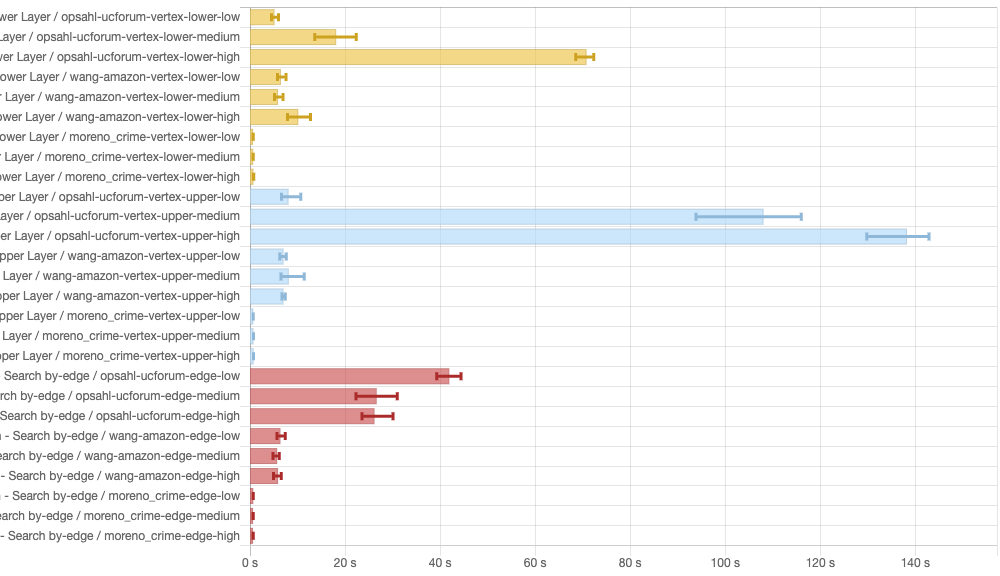
\includegraphics[width=\textwidth]{bench_1.png}
  \captionsetup{type=figure}
  \captionof{figure}{Benchmark 1 - DP in Haskell vs. Data.Graph Haskell}
  \label{fig:1}
\end{minipage}

\autoref{fig:1} shows that $DP_{WCC}$ in Haskell solution is $1.3$ faster compare with \acrshort{hs} \texttt{containers} library. Despite this, if we zoom  in \autoref{fig:1}, it can be observed that $DP_{WCC}$ in Haskell solution is slower compared with \acrshort{hs} \texttt{containers}; the reasons behind this have been explained in \autoref{sub:sec:e1}.
\iffalse
\begin{minipage}[t]{\linewidth}
  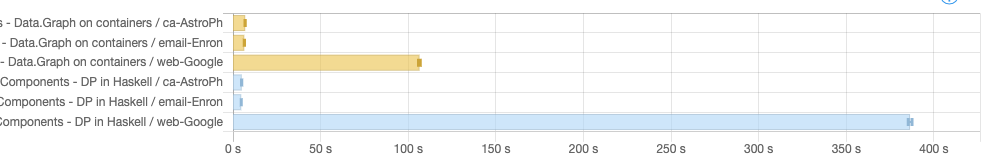
\includegraphics[width=\textwidth]{bench_2}
  \captionsetup{type=figure}
  \captionof{figure}{Benchmark 2 - DP in Haskell vs. Data.Graph Haskell}
  \label{fig:2}
\end{minipage}
\fi

Regarding mean execution times for each implementation on each case measure by \texttt{criterion} library \cite{criterion}, we can display the following results:

\begin{table}[H]
  \centering
  \begin{tabular}{|l|l|l|l|}
   \hline
   \textbf{Network} & \textbf{$DP_{WCC}$ in Haskell} & \textbf{\acrshort{hs} \texttt{containers}} & \textbf{Speed-up}\\
   \hline
   Enron Emails & 4.68s &  6.46s & 1.38\\
   \hline
   Astro Physics Coll Net & 4.98s & 6.95s  & 1.39\\
   \hline
   Google Web Graph & 386s & 106s & -3.64\\
   \hline
  \end{tabular}
 \caption{Mean Execution times}
 \label{table:6}
 \end{table}

These results allow for answering Question [Q2].
We already had a partial answer with the previous experiment E1 about [Q2] (\autoref{res:question}) where we have seen that the graph topology is affecting the performance and the parallelization, penalizing $DP_{WCC}$ in Haskell for this particular case. In this benchmark, the solution against a non-parallel \texttt{containers} \mintinline{haskell}{Data.Graph} confirms the hypothesis. 

\paragraph{Diefficency Metrics}\label{sub:sub:sec:e2}
Some considerations are needed before starting to analyze the data gathered with \acrshort{dm} tool. Firstly, the tool is plotting the results according to the traces generated by the implementation, both $DP_{WCC}$ in Haskell  and \acrshort{hs} \emph{containers}. By the nature of \acrshort{dp} model, we can gather or register that timestamps as long as the model is generating results. In the case of \acrshort{hs} \texttt{containers}, this is not possible since it calculates \acrshort{wcc} at once. This is not an issue and we still can check at what point in time all \acrshort{wcc} in \acrshort{hs} \texttt{containers} are generated. In those cases, we are going to see a straight vertical line. 

It is important to remark that we needed to scale the timestamps because we have taken the time in nanoseconds. After all, the incremental generation between one \acrshort{wcc} and the other is very small but significant enough to be taken into consideration. Thus, if we left the time scale in integer milliseconds, microseconds, or nanoseconds integer part it cannot be appreciated. In case of escalation, we are discounting the nanosecond integer of the first generated results resulting in a time scale that starts close to $0$. This does not mean that the first result is generated at $0$ time, but we are discarding the previous time to focus on how the results are incrementally generated.

Having said that, we can see the results of \acrshort{dm} which are presented in two types of plots. The first one is regular line graphs in where the $x$ axis shows the time escalated when the result was generated and the $y$ axis is showing the component number that was generated at that time. The second type of plot is a radar plot in which shows how the solution is behaving on the dimensions of  \acrfull{tfft}, \acrfull{et}, \acrfull{tt}, \acrfull{comp} and \acrfull{dt} and how are the tension between them; all these metrics are higher is better. All the details about these metrics are explained here \cite{diefpaper}.

\begin{figure}[!htb]
    \centering
    \begin{minipage}{0.33\textwidth}
     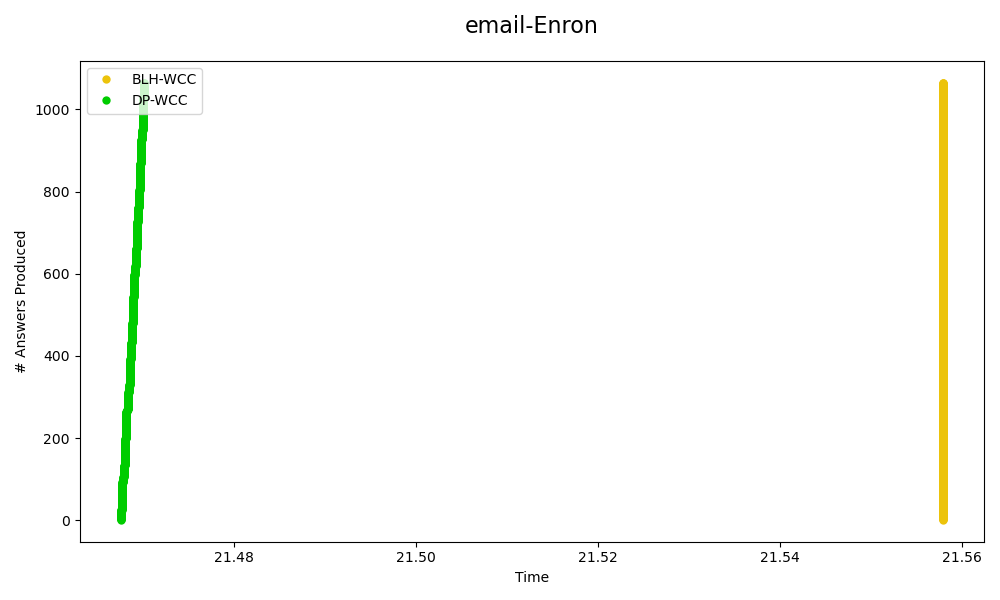
\includegraphics[width=1\linewidth, height=0.2\textheight]{email_enron0}
      \caption{email-Enron \acrshort{dm}}
      \label{fig:dief:1}
    \end{minipage}%
    \begin{minipage}{0.33\textwidth}
     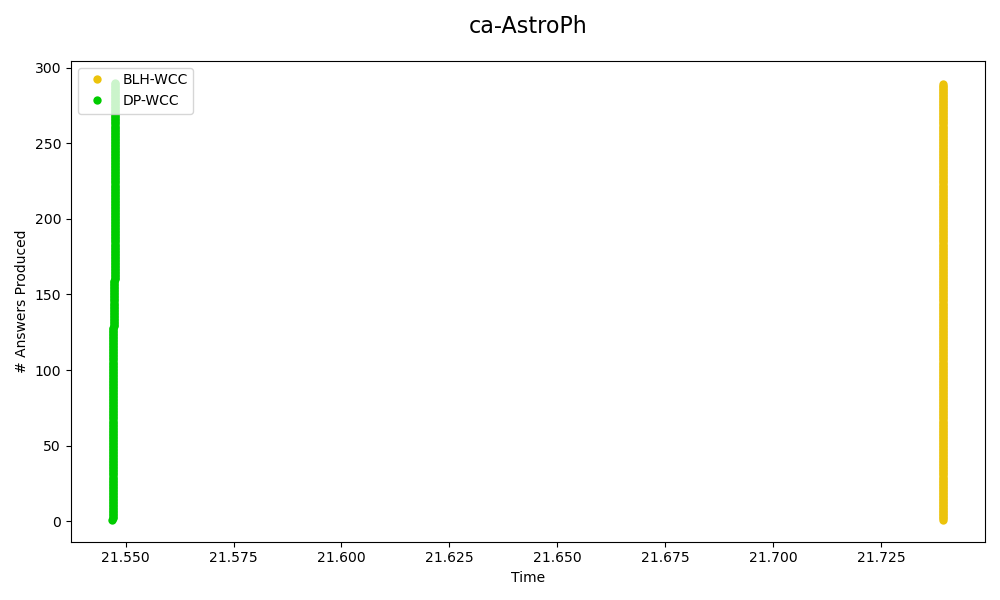
\includegraphics[width=1\linewidth, height=0.2\textheight]{ca_astroph0}
      \caption{ca-AstroPh \acrshort{dm}}
      \label{fig:dief:2}
    \end{minipage}%
    \begin{minipage}{0.33\textwidth}
     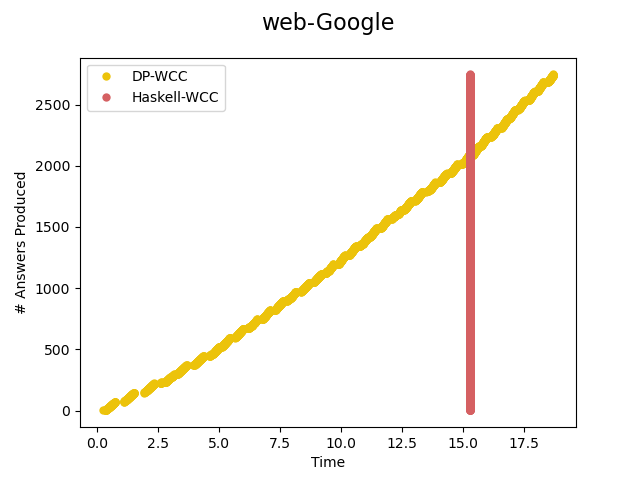
\includegraphics[width=1\linewidth, height=0.2\textheight]{web_google0}
      \caption{web-Google \acrshort{dm}}
      \label{fig:dief:3}
    \end{minipage}
\end{figure}

Based on the results shown in all the figures above, all the solutions in $DP_{WCC}$ in Haskell are being generated incrementally, but there is some difference that we would like to remark. In the case of \emph{email-Enron} and \emph{ca-AstroPh} graphs as we can see in \autoref{fig:dief:1} and \autoref{fig:dief:2}, there seems to be a more incremental generation of results. This is behavior is measured with the values of \acrfull{dt}. \emph{ca-AstroPh} as it can be seen in \autoref{fig:dief:2}, is even more incremental showing a clear separation between some results and others. The \emph{web-Google} network which is shown in \autoref{fig:dief:3}, is a little more linear and that is because all the results are being generated with very little difference in time between them. This is due to the fact of the explained reasons in \autoref{sub:sec:e1}. Having the biggest \acrshort{wcc} at the end of \emph{web-Google}, \acrshort{dp} algorithm it is retaining results until the biggest \acrshort{wcc} can be solved, which takes longer. 

\begin{figure}[!htb]
    \centering
    \begin{minipage}{0.33\textwidth}
     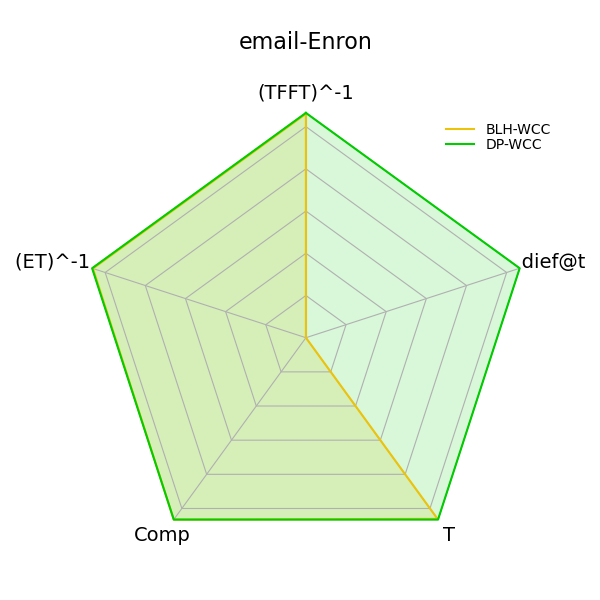
\includegraphics[width=1\linewidth, height=0.2\textheight]{email_enron_radar0}
      \caption{email-Enron \acrshort{dm}}
      \label{fig:dief:rad:1}
    \end{minipage}%
    \begin{minipage}{0.33\textwidth}
     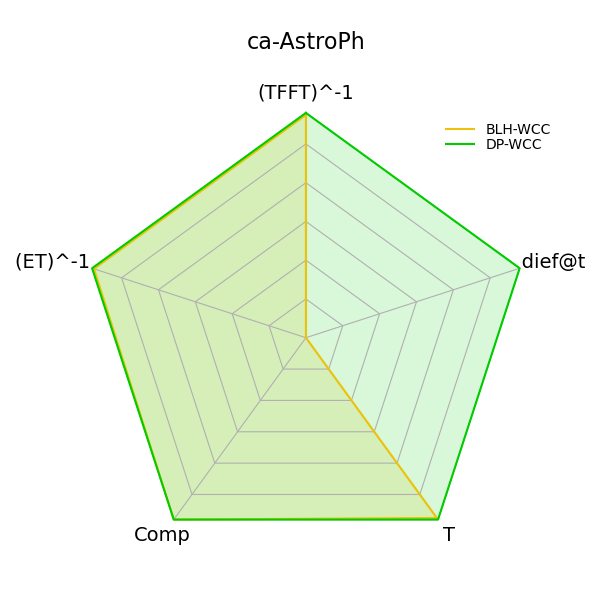
\includegraphics[width=1\linewidth, height=0.2\textheight]{ca_astroph_radar0}
      \caption{ca-AstroPh \acrshort{dm}}
      \label{fig:dief:rad:2}
    \end{minipage}%
    \begin{minipage}{0.33\textwidth}
     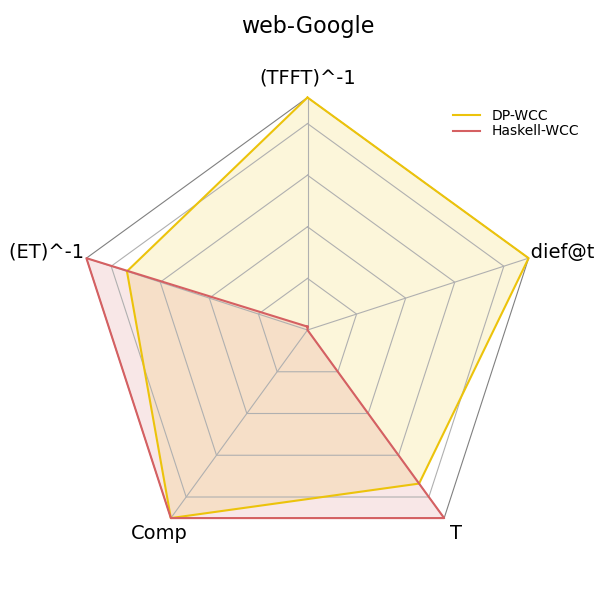
\includegraphics[width=1\linewidth, height=0.2\textheight]{web_google_radar0}
      \caption{web-Google \acrshort{dm}}
      \label{fig:dief:rad:3}
    \end{minipage}
\end{figure}

As we can appreciate in the above radar plots our previous analysis can be confirmed. We can see for example that the \acrlong{tt} of \emph{web-Google} in \autoref{fig:dief:rad:3}, in the case of $DP_{WCC}$ in Haskell is worse than \acrshort{hs} \texttt{containers}, which is not happening for the others.

In conclusion, we can say that regarding [Q2] (\autoref{res:question}) although $DP_{WCC}$ in Haskell is faster than the traditional approach, the speed-up dimension execution factor is not always the most interest analysis that we can have, because as we have seen even when in the case of \emph{web-Google} Graph $DP_{WCC}$ in Haskell is slower at execution, it is at least generating incremental results without the need to wait for the rest of the computations.

\paragraph{Experiment: E3}
For this type of analysis, our experiment focuses on \emph{email-Enron} network \cite{netenron} only because profiling data generated by \acrshort{ghc} is big enough to conduct the analysis and on the other, and enabling profiling penalize execution time.

\paragraph{Multithreading} For analyzing parallelization and multithreading we have used \textit{ThreadScope} \cite{threadscope} which allows us to see how the parallelization is taking place on \acrshort{ghc} at a fine grained level and how the threads are distributed throughout the different cores requested with the \mintinline{bash}{-N} execution \texttt{ghc-option} flag.

\begin{minipage}[t!]{\linewidth}

  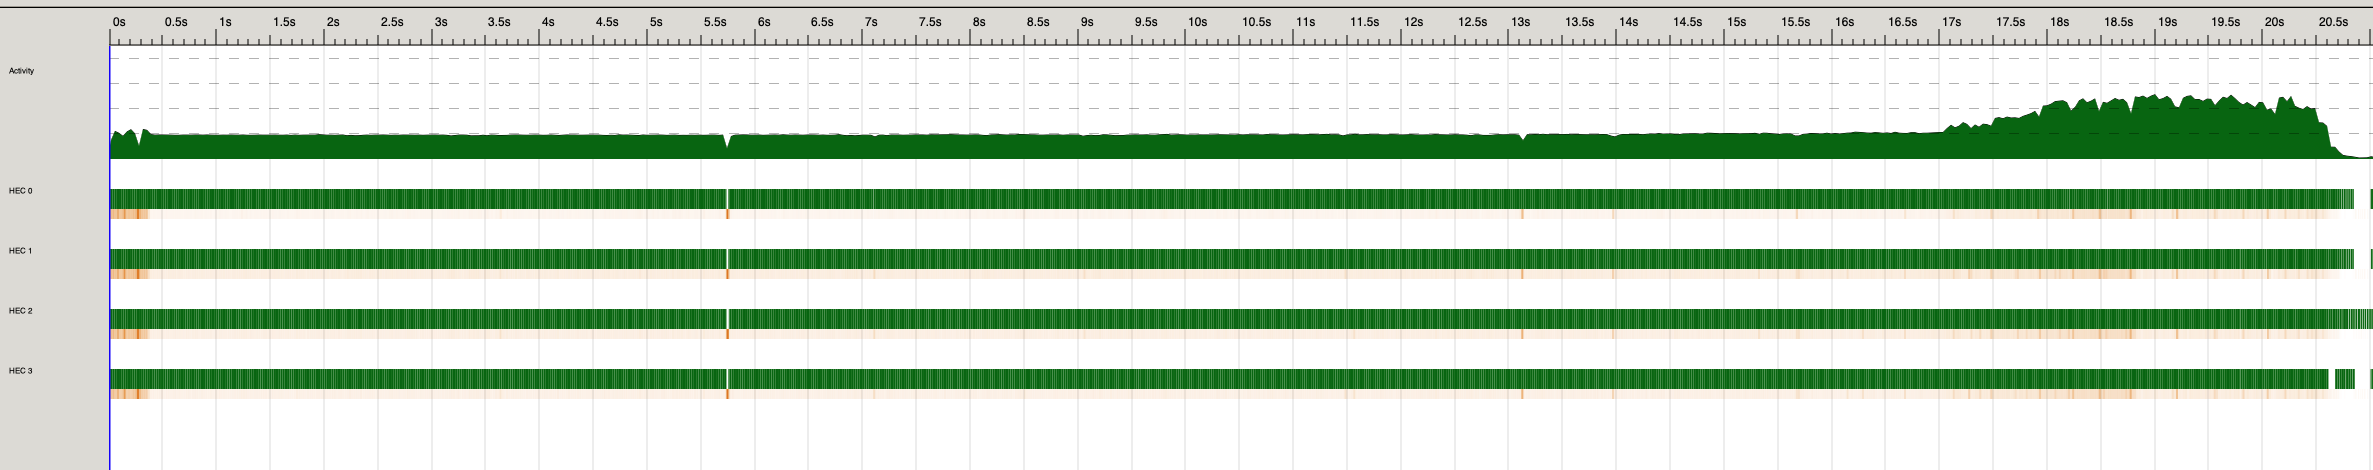
\includegraphics[width=\textwidth]{screen_1}
  \captionsetup{type=figure}
  \captionof{figure}{Threadscope Image of General Execution}
  \label{fig:3}
\end{minipage}

In \autoref{fig:3}, we can see that the parallelization is being distributed evenly among the $4$ Cores that we have set for this execution.
The distribution of the load is more intensive at the end of the execution, where \mintinline{haskell}{actor2} filter stage 
%as it can be seen in \autoref{src:haskell:3}, 
of the algorithm is taking place and different filters are reaching execution of that second actor.

\begin{wrapfigure}{r}{0.5\textwidth}
  \begin{center}
     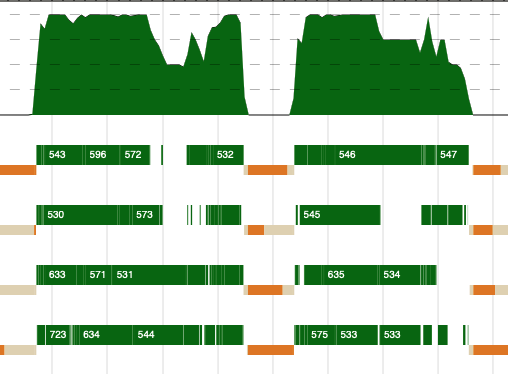
\includegraphics[width=0.48\textwidth] {screen_2}
     %[width=10cm, height=9cm]
       \end{center}
     \caption{Threadscope Image of Zoomed Fraction}
     \label{fig:4}
 %\end{figure}
 \end{wrapfigure}
Another important aspect shown in \autoref{fig:3}, is that this work is not so significant for \acrshort{ghc} and the threads and distribution of the work keeps between 1 or 2 cores during the execution time of the \mintinline{haskell}{actor1}. However, the usages increase on the second actor as pointed out before. In this regard, we can answer research questions [Q1] and [Q3] (\autoref{res:question}), verifying that \acrshort{hs} not only supports the required parallelization level but is evenly distributed across the program execution too.

Finally, it can also be appreciated that there is no sequential execution on any part of the program because the $4$ cores have \textit{CPU} activity during the whole execution time. This is because as long the program start, and because of the nature of the \acrshort{dp} model, it is spawning the \textit{Source} stage in a separated thread. This is a clear advantage for the model and the processing of the data since the program does not need to wait to do some sequential processing like reading a file, before start computing the rest of the stages.


\autoref{fig:4} zooms in on \textit{ThreadScope} output in a particular moment, approximately in the middle of the execution. We can appreciate how many threads are being spawned and by the tool and if they are evenly distributed among cores. The numbers inside green bars represent the number of threads that are being executed on that particular core (horizontal line) at that execution slot. Thus, the number of threads varies among slot execution times because as it is already known, \acrshort{ghc} implements \emph{Preemptive Scheduling} \cite{lightweightghc}.

Having said that, it can be appreciated in \autoref{fig:4} our first assumption that the load is evenly distributed because the mean number of executing threads per core is $571$.

\paragraph{Memory allocation} Another important aspect in our case is how the memory is being managed to avoid memory leaks or other non-desired behavior that increases memory allocation during the execution time. This is even more important in the particular implementation of \acrshort{wcc} using \acrshort{dp} model because it requires to maintain the set of connected components in memory throughout the execution of the program or at least until we can output the calculated \acrshort{wcc} if we reach to the last \textit{Filter} and we know that this \acrshort{wcc} cannot be enlarged anymore. 

In order to verify this, we measure memory allocation with \textit{eventlog2html} \cite{eventlog2html} which converts generated profiling memory eventlog files into graphical HTML representation. 

\begin{wrapfigure}{r}{0.5\textwidth}
  \begin{center}
     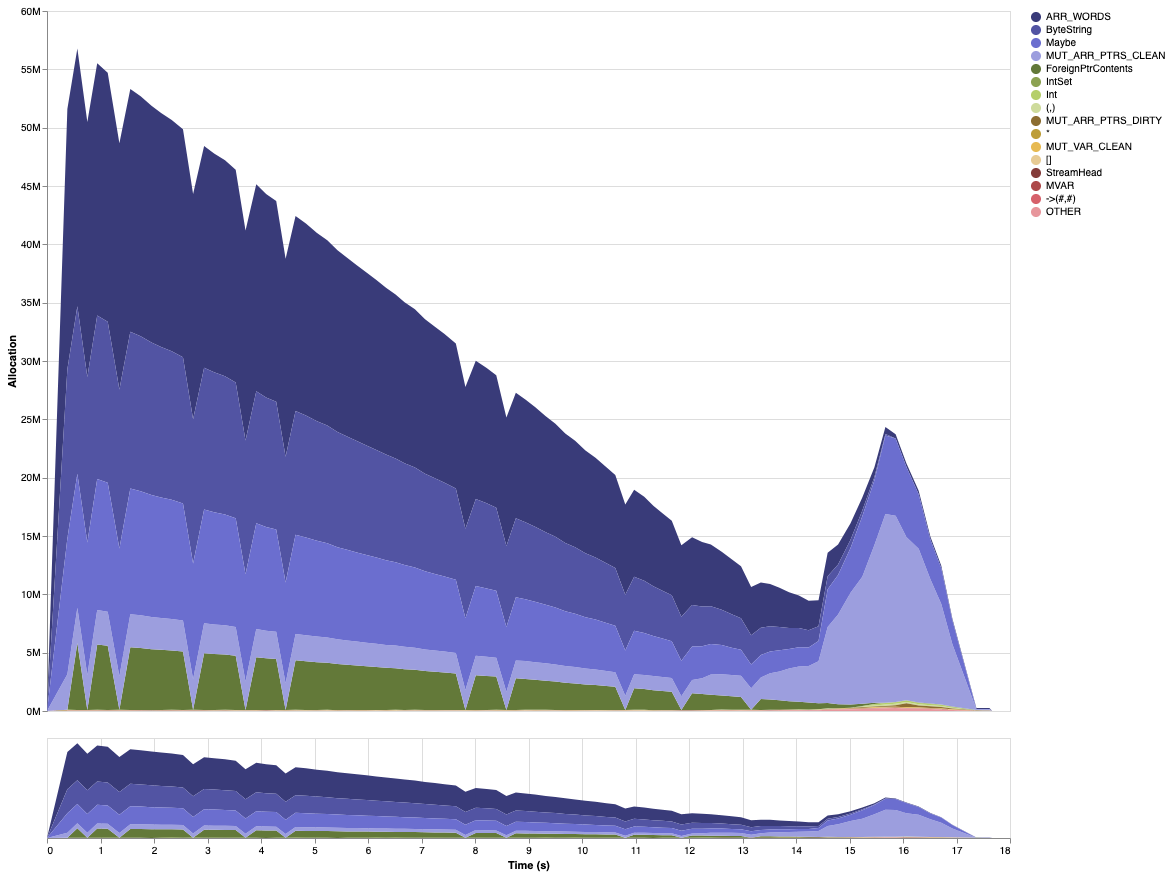
\includegraphics[width=0.5\textwidth] {visualization}
     %[width=10cm, height=9cm]
       \end{center}
     \caption{Memory Allocation}
     \label{fig:5}
 %\end{figure}
 \end{wrapfigure}

As we can see in \autoref{fig:5}, $DP_{WCC}$ in Haskell does an efficient work on allocating memory since we are not using more than $57$ MB of memory during the whole execution of the program.

On the other hand, if we analyze how the memory is allocated during the execution of the program, it can also be appreciated that most of the memory is allocated at the beginning of the program and steadily decrease over time with a small peak at the end that does not overpass even half of the initial peak of $57$ MB. The explanation for this behavior is quite straightforward because at the beginning we are reading from the file and transforming a \mintinline{haskell}{ByteString} buffer to \mintinline{haskell}{(Int, Int)} edges. This is seen in the image in which the dark blue that is on top of the area is \mintinline{haskell}{ByteString} allocation. Light blue is allocation of \mintinline{haskell}{Maybe a} type which is the type that is returned by the \textit{Channels} because it can contain a value or not. Data value \mintinline{haskell}{Nothing} is indicating end of the \textit{Channel}. 

Another important aspect is the green area which represents \mintinline{haskell}{IntSet} allocation, which in the case of our program is the data structure that we use to gather the set of vertices that represents a \acrshort{wcc}. This means that the amount of memory used for gathering the \acrshort{wcc} itself is minimum and it is decreasing over time, which is another empirical indication that we are incrementally releasing results to the user. It can be seen as well that as long the green area reduces the lighter blue (\mintinline{haskell}{MUT_ARR_PTRS_CLEAN} \cite{ghcheap}) increases at the same time indicating that the computations for the output (releasing results) is taking place. 

Finally, according to what we have stated above, we can answer the question [Q3] (\autoref{res:question}) showing that not only memory management was efficient, but at the same time, the memory was not leaking or increasing across the running execution program.

The empirical evaluation of the $DP_{WCC}$ in Haskell to compute weakly connected components of a graph, evidences  suitability, and robustness of this  language to of  support the development of a Dynamic Pipeline Framework. Measuring using diefficienc metrics reveals some advantageous capability of $\dpwcc$ implementation to deliver incremental results compared with default containers library implementation.  Regarding the main aspects where DPP is strong, i.e., pipeline parallelism and time processing, the $\dpwcc$ performance shows that Haskell can deal with the requirements for the \acrshort{wcc} problem without penalizing neither execution time nor memory allocation. In particular, the $\dpwcc$ implementation outperforms in those cases where the topology of the graph is sparse and where the number of vertices in the largest \acrshort{wcc} is not big enough.  

To conclude, the proof of concept has gathered enough evidence to show that the implementation of a Dynamic Pipeline solutions in Haskell Programming Language is feasible. This fact opens a wide range of algorithms to be explored using the Dynamic Pipeline Paradigm, supported by purely functional programming language. This results give us insights about how to proceed for implementing a first version of a DPF using (parallel) Haskell.
The empirical study aims at evaluating $\dpwcc$ implemented in the baseline \acrshort{hs} and \acrshort{dpfh}. Our goal is to answer the following research questions: 

\begin{inparaenum}[\bf {\bf RQ}1\upshape)]
\label{res:question}
    \item Does \acrshort{dpfhwcc} exhibit similar execution time performance compared with \acrshort{dpwcc}?
    \item Does \acrshort{dpfhwcc} enhance the continuous behavior with respect to other approaches?
    \item Do the proposed approaches to $\dpwcc$ handle memory efficiently?
\end{inparaenum}

We have implemented three solutions to the problem of weakly connected components:
\begin{itemize}
\item \acrshort{blwcc}: implemented in \texttt{containers} \acrshort{hs} library \footnote{\url{https://hackage.haskell.org/package/containers}} using \mintinline{haskell}{Data.Graph}.
\item \acrshort{dpwcc}: baseline implementation of the weakly connected components as a dynamic pipeline (\autoref{prole}).
\item \acrshort{dpfhwcc}: implementation of the weakly connected components on top of the DPF-Haskell framework (\autoref{sec:wcc-dpf}). 
\end{itemize}

\paragraph{Running Architecture}
All the experiments have been executed in a $x86$ $64$ bits architecture with a \textit{$6$-Core Intel Core i7} processor of $2,2$ GHz, which can emulate up to $12$ virtual cores. This processor has \emph{hyper-threading} enable. Regarding memory, the machine has $32 GB$ \emph{DDR4} of RAM, $256\ KB$ of L2 cache memory, and $9\ MB$ of L3 cache.

\paragraph{Haskell Setup}
We have used the following \acrshort{hs} setup for \acrshort{dpwcc} implementation: \acrshort{ghc} version $8.10.4$, \mintinline[breaklines]{bash}{bytestring 0.10.12.0}\footnote{\url{https://hackage.haskell.org/package/bytestring}}, \mintinline[breaklines]{bash}{containers 0.6.2.1}\footnote{\url{https://hackage.haskell.org/package/containers}}, \mintinline[breaklines]{bash}{relude 1.0.0.1}\footnote{\url{https://hackage.haskell.org/package/containers}} and \mintinline[breaklines]{bash}{unagi-chan 0.4.1.3}\footnote{\url{https://github.com/jberryman/unagi-chan}}. 
The use of \texttt{relude} library is because we disabled \mintinline{haskell}{Prelude} from the project with the language extension (language options) \mintinline[breaklines]{haskell}{NoImplicitPrelude}\footnote{\url{https://downloads.haskell.org/ghc/8.8.4/docs/html/users_guide/}}. 
Regarding compilation flags (\acrshort{ghc} options) we have compiled our program with \mintinline[breaklines]{bash}{-threaded}, \mintinline[breaklines]{bash}{-O3}, \mintinline[breaklines]{bash}{-rtsopts}, \mintinline[breaklines]{bash}{-with-rtsopts=-N}. 
Since we have used \texttt{stack} version $2.5.1$ \footnote{\url{https://docs.haskellstack.org/en/stable/README/}} as a building tool on top of \acrshort{ghc} the compilation command is \mintinline[breaklines]{bash}{stack build}\footnote{For more information about package.yaml or cabal file please check \url{https://github.com/jproyo/upc-miri-tfm/tree/main/connected-comp}}.
Additionally, the setup for \acrshort{dpfhwcc} is the same as the exposed before but with the difference that this setup use \mintinline[breaklines]{bash}{dynamic-pipeline 0.3.2.0}\footnote{\url{https://hackage.haskell.org/package/dynamic-pipeline}} library written in the context of this work.


\paragraph{DataSets}\label{data:set}
For all the experiments, we have used the following networks taken from \acrshort{snap} \cite{stanford}. %In this particular experiment setup, we have selected the following specific data sets that can be found here \cite{netastro, netenron, netwebgoogle}

\begin{table}[H]
  \centering
  \begin{tabular}{|p{0.25\linewidth}|r|r|r|r|r|}
   \hline
   \textbf{Network} & \textbf{Nodes} & \textbf{Edges} & \textbf{Diameter} & \textbf{\#\acrshort{wcc}} & \textbf{\#Nodes Largest WCC} \\
   \hline
   Enron Emails & 36,692 & 183,831 & 11 & 1,065 & 33,696 (0.918) \\
   \hline
   Astro Physics Collaboration Net & 18,772 & 198,110 & 14 & 290 & 17,903 (0.954)\\
   \hline
   Google Web Graph & 875,713 & 5,105,039 & 21 & 2,746 & 855,802 (0.977)\\
   \hline
  \end{tabular}
 \caption{DataSet of Graphs Selected}
 \label{table:4}
 \end{table}
 
 The criteria for selecting the networks have been followed the idea or testing the solution in more complex graphs, in which all of them are undirected graphs but with different sizes concerning its number of nodes as we can see in  \autoref{table:4}. 
 
 \iffalse
have conducted different kinds of experiments to test our assumptions.
First, we have used graphs from \acrfull{snap} \cite{stanford} and analyze how three implementations of the problem weakly connected components behave under real-world graphs. 

if it timeouts or not and if it is producing correct results in terms of the amount of \acrshort{wcc} that we know beforehand.
We have also tested the implementation doing a \emph{Benchmark Analysis} where we focus on two different types of benchmarks. On the one hand, using \texttt{criterion} library \footnote{\url{https://hackage.haskell.org/package/criterion}}, we have evaluated a benchmark between our solution and \acrshort{wcc} algorithm implemented in \texttt{containers} \acrshort{hs} library \cite{containers} using \mintinline{haskell}{Data.Graph}. On the other hand, we have compared if the results are being generated incrementally in both cases and how that is done during the pipeline execution time. This last analysis has been conducted using \texttt{diefpy} tool.
Finally, we have executed a \textit{Performance Analysis} in which we have to gather profiling data from \acrfull{ghc} for one of the real-world graphs, to measure how the program performs regarding multithreading and memory allocation.


In order to answer the former questions, we have conducted the same experiments that we did on \textit{Proof of Concept} evaluation, but not focusing on the comparison with default \acrshort{hs} \texttt{containers} implementation. 
Another topic that we haven't measured in this empirical analysis is the performance of \textit{Memory and Threads} allocation. 
The networks selected for this evaluation are the same as the networks used on \autoref{prole}.

\paragraph{Running Architecture}
All the experiments have been executed in a $x86$ $64$ bits architecture with a \textit{$6$-Core Intel Core i7} processor of $2,2$ GHz which can emulate up to $12$ virtual cores. This processor has \emph{hyper-threading} enable. Regarding memory, the machine has $32 GB$ \emph{DDR4} of RAM, $256\ KB$ of L2 cache memory, and $9\ MB$ of L3 cache.

\paragraph{Haskell Setup}
Regarding specific libraries and compilations flags used on \acrshort{hs}, we have used \acrshort{ghc} version $8.10.4$. 
We have also used the following set of libraries: \mintinline{bash}{bytestring 0.10.12.0} \cite{bytestring}, \mintinline{bash}{containers 0.6.2.1} \cite{containers}, \mintinline{bash}{relude 1.0.0.1} \cite{relude} and \mintinline{bash}{dynamic-pipeline 0.3.2.0} \cite{dynamic-pipeline}. 
The use of \texttt{relude} library is because we disabled \mintinline{haskell}{Prelude} from the project with the language extension \mintinline{haskell}{NoImplicitPrelude} \cite{extensions}. 
Regarding compilation flags (\acrshort{ghc} options) we have compiled our program with \mintinline{bash}{-threaded}, \mintinline{bash}{-O3}, \mintinline{bash}{-rtsopts}, \mintinline{bash}{-with-rtsopts=-N}. 
Since we have used \texttt{stack} version $2.5.1$ \cite{stack} as a building tool on top of \acrshort{ghc} the compilation command is \mintinline{bash}{stack build}\footnote{For more information about package.yaml or cabal file please check https://github.com/jproyo/upc-miri-tfm/tree/main/connected-comp}.
\fi

\subsection{Experiments Definition}\label{sub:new:exp:def}
\paragraph{E1: Implementation Analysis}
In this experiment, we measure \acrshort{ghc} statistics running time enabling \mintinline{bash}{+RTS -s} flags. The metrics that we measure are \emph{MUT Time} which is the amount of time in seconds \acrshort{ghc} is running computations and \emph{GC Time} which is the number of seconds that \acrshort{ghc} is running garbage collector. \emph{Total execution time} is the sum of both in seconds. At the same time, we are going to check the correctness of the output counting the number of \acrshort{wcc} generated by the algorithm against the already known topology of it in \autoref{data:set}. 
Similarly, in this experiment, we measure \acrshort{ghc} statistics running time enabling \mintinline{bash}{+RTS -s} flags.
The metrics that we measure are \emph{MUT Time} which is the amount of time in seconds \acrshort{ghc} is running computations and \emph{GC Time} which is the number of seconds that \acrshort{ghc} is running garbage collector. 
\emph{Total execution time} is the sum of both in seconds. The experiment provides evidence to answer the research question [RQ2].

\paragraph{E2: Benchmark Analysis}
This experiment measures \emph{Average Running Time}.
The \emph{Average Running Time} is the average running time of $1000$ resamples using \texttt{criterion} tool. 
In each sample, the running time is measure from the beginning of the execution of the program until when the last answer is produced.
This experiment will help to answer research question [RQ1].

\paragraph{E3: Continuous Behavior - Diefficiency Metrics}
In this experiment, we conduct two benchmark analysis over execution time comparing \acrshort{dpwcc} vs. \acrshort{blwcc}. 
In the first benchmark analysis, we use \texttt{criterion} tool in \acrshort{hs} which runs over four iterations of each of the algorithms to get a mean execution time in seconds and compare the results in a plot. 
In the second benchmark, we use \acrfull{dm} Tool \acrshort{dtkp} in order to measure with the ability of \acrshort{dp} model to generate results incrementally \cite{diefpaper}. 
This is one of the strongest feature of \acrshort{dp} Paradigm since it allows process and generate results without no need of waiting for processing until the last element of the data source. 
This kind of aspect is essential not only for big data inputs where perhaps the requirements allow for processing until some point of the time having partial results but at the same time is important to process unbounded streams.
This experiment measures \acrlong{dm} described in \autoref{prem:dief}, and will help to answer research question [RQ2].

\paragraph{E4: Performance Analysis}
In this experiment, we measure internal parallelism in \acrshort{ghc} and memory usage during the execution of one of the example networks. 
The motivation of this is to verify empirically how \acrshort{dpwcc} is handling parallelization and memory usage. 
This experiment is conducted using two tools, \textit{ThreadScope} Tool\footnote{\url{https://wiki.haskell.org/ThreadScope}} for conducting multithreading analysis and \textit{eventlog2html} Tool\footnote{\url{https://mpickering.github.io/eventlog2html/}} to conduct memory usage analysis. 
Regarding multithreading analysis the metrics that we measure are the distribution of threads among processors over execution time which is how many processors are executing running threads over the whole execution; and the mean number of running threads per time slot which is calculated by zooming in $8$ time slots and taking the mean number of threads per processor to see if it is equally distributed among them. 
In regards to memory management, the metric that we measure is the amount of memory in $MB$ consumed per data type during the whole execution time. 
The experiment helps to answer the research questions [RQ1,RQ3].

\subsection{Discussion of Observed Results}\label{new:experiments}
\paragraph{Experiment: E1}\label{sub:new:sec:e1}
The following represents the execution for running these graphs on our \acrshort{dp} implementation.

\begin{table}[H]
  \centering
  \begin{tabular}{|l|r|r|r|r|}
   \hline
   \textbf{Network} & \textbf{Exec Param} & \textbf{MUT Time} & \textbf{GC Time} & \textbf{Total Time}\\
   \hline
   Enron Emails & \mintinline{bash}{+RTS -N4 -s} & 2.797s & 0.942s & 3.746s \\
   \hline
   Astro Physics Coll Net & \mintinline{bash}{+RTS -N4 -s} & 2.607s & 1.392s & 4.014s \\
   \hline
   Google Web Graph & \mintinline{bash}{+RTS -N8 -s} & 137.127s & 218.913s & \textbf{\textcolor{red}{356.058s}} \\
   \hline
  \end{tabular}
  \caption{Total Execution times of each of the networks implemented with \acrshort{dpwcc}. \textit{MUT Time} is the time of running or executing code and \textit{GC Time} is the time that the program spent doing Garbage collection. \textit{Total Execution time} is the sum of both times}
 \label{table:5}
 \end{table}

It is important to point out that since the first two networks are smaller in the number of edges compared with \emph{web-Google}, executing those with $8$ cores as the \mintinline{bash}{-N} parameters indicates, does not affect the final speed-up since \acrshort{ghc} is not distributing threads on extra cores because it handles the load with $4$ cores only.

As we can see in \autoref{table:5}, we are obtaining remarkable execution times for the first two graphs and it seems not to be the case for \textit{web-Google}. Doing a deeper analysis on the topology of this last graph, we can see according to \autoref{table:4} that the number of \textit{Nodes in the largest \acrshort{wcc}} is the highest one. This means that there is a \acrshort{wcc} which contains $97.7\%$ of the nodes. Moreover, we can confirm that if we analyze even deeper how is the structure of that \acrshort{wcc} with the output of the algorithm, we can notice that the largest \acrshort{wcc} is the last one on being processed. Having that into consideration we can state that due to the nature of our algorithm which needs to wait for collecting all the vertices in the \mintinline{haskell}{actor2} filter stage 
%as it can be seen in \autoref{src:haskell:3}, 
it penalizes our execution time for that particular case. A more elaborated technique for implementing the actors is required to speed up execution. 

Regarding the correctness of the output, we have verified with the outputs that the number of connected components is the same as the metrics already gathered in \autoref{table:4}.

The following represents the \emph{Total execution time} for each of the networks implemented with \acrshort{dpfhwcc}.
 
\begin{table}[H]
  \centering
  \begin{tabular}{|l|r|r|r|r|}
   \hline
   \textbf{Network} & \textbf{Exec Param} & \textbf{MUT Time} & \textbf{GC Time} & \textbf{Total Time}\\
   \hline
   Enron Emails & \mintinline{bash}{+RTS -N4 -s} & 1.795s & 0.505s & 2.314s \\
   \hline
   Astro Physics Coll Net & \mintinline{bash}{+RTS -N4 -s} & 2.294s & 1.003s & 3.311s \\
   \hline
   Google Web Graph & \mintinline{bash}{+RTS -N8 -s} & 169.381s & 270.784s & 440.176s \\
   \hline
  \end{tabular}
 \caption{Total Execution times of each of the networks implemented with \acrshort{dpfhwcc}. \textit{MUT Time} is the time of running or executing code and \textit{GC Time} is the time that the program spent doing Garbage collection. \textit{Total Execution time} is the sum of both times}
 \label{table:new:wcc:dpfh:5}
 \end{table}

In \autoref{table:new:wcc:dpfh:5}, we are obtaining similar execution times compared with \autoref{table:5} in \autoref{prole}.
In fact, for \textit{Enron Emails} and \textit{Astro Physics Coll} networks, all times are better than the implementation of the \textit{Proof of Concept}.
Regarding \textit{Google Web} network, the time is slightly worse but there is the fact that \acrshort{dpfh} is adding some overhead over plain code execution.
According to these results we can partially answer [RQ1], because the implementation of \acrshort{dpfhwcc} has similar performance compared with \textit{Proof of Concept} implementation. 

\paragraph{Experiment: E2}\label{sub:new:exp:2}
\paragraph{Criterion Benchmark}
In \autoref{fig:1}, orange bars report the time taken by \mintinline{haskell}{Data.Graph} in $DP_{WCC}$ in Haskell \texttt{containers} library\footnote{\url{https://hackage.haskell.org/package/containers}}. Blue light bars represent the time taken by $DP_{WCC}$ in Haskell.

\begin{minipage}[t]{\linewidth}
  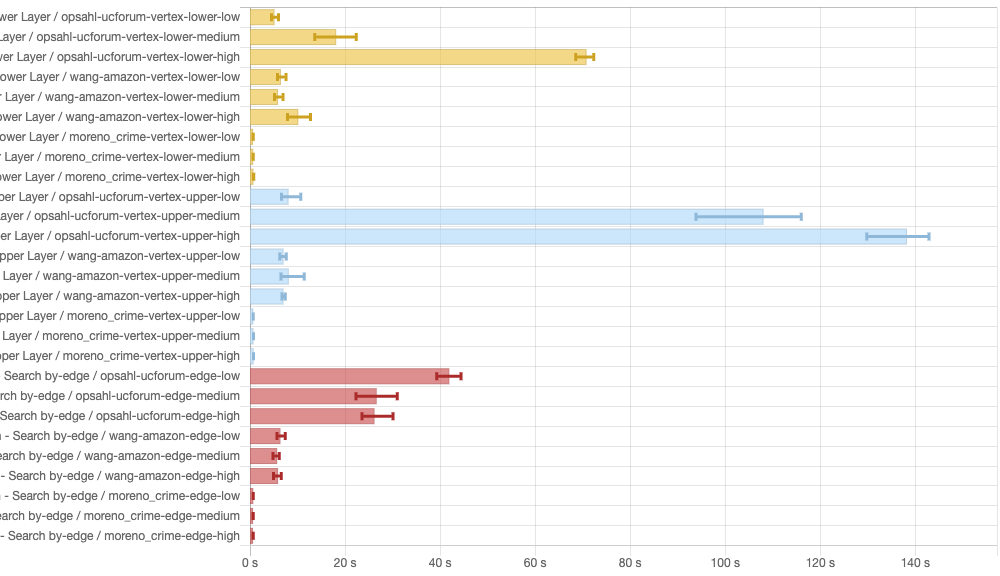
\includegraphics[width=\textwidth]{bench_1.png}
  \captionsetup{type=figure}
  \captionof{figure}{Benchmark of average execution time of \acrshort{dpwcc} vs. \acrshort{blwcc}. Average Execution time of running $1000$ samples over each of the networks.}
  \label{fig:1}
\end{minipage}

\autoref{fig:1} shows that \acrshort{dpwcc} solution is $1.3$ faster compare with \acrshort{blwcc}. 
Despite this, if we zoom  in \autoref{fig:1}, it can be observed that \acrshort{dpwcc} solution is slower compared with \acrshort{blwcc}.
Regarding mean execution times for each implementation on each case measure by \texttt{criterion} library, we can display the following results:

\begin{table}[H]
  \centering
  \begin{tabular}{|l|l|l|l|}
   \hline
   \textbf{Network} & \textbf{\acrshort{dpwcc}} & \textbf{\acrshort{blwcc}} & \textbf{Speed-up}\\
   \hline
   Enron Emails & 4.68s &  6.46s & 1.38\\
   \hline
   Astro Physics Coll Net & 4.98s & 6.95s  & 1.39\\
   \hline
   Google Web Graph & 386s & 106s & -3.64\\
   \hline
  \end{tabular}
 \caption{Comparison of Mean Execution times between \acrshort{dpwcc} vs. \acrshort{blwcc} for each network}
 \label{table:6}
 \end{table}

These results allow for answering Question [Q2].
We already had a partial answer with the previous experiment E1 about [Q2] (\autoref{res:question}) where we have seen that the graph topology is affecting the performance and the parallelization, penalizing \acrshort{dpwcc} for this particular case. 
In this benchmark, the solution against \acrshort{blwcc} confirms the hypothesis. 

Moreover, \autoref{fig:new:1}, we can appreciate the \textit{Average Execution Time} for each of the networks after running \texttt{criterion} tool for the \acrshort{dpfhwcc} implementation confirming that after changing the \acrshort{dp} implementation using \acrshort{dpfh} the performance remains stable.

\begin{minipage}[t]{\linewidth}
  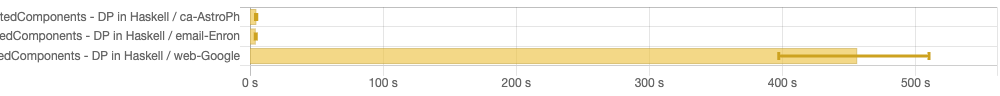
\includegraphics[width=\textwidth]{bench_1_new.png}
  \captionsetup{type=figure}
  \captionof{figure}{Average Execution time of running $1000$ samples over each of the networks with \acrshort{dpfhwcc} implementation.}
  \label{fig:new:1}
\end{minipage}

If we compare those \textit{Average Execution Times} with the previous obtained in \autoref{prole}, we have the following comparison table.

 \begin{table}[H]
  \centering
  \begin{tabular}{|l|l|l|l|}
   \hline
   \textbf{Network} & \textbf{\acrshort{dpfhwcc}} & \textbf{\acrshort{dpwcc}} & \textbf{Speed-up}\\
   \hline
   Enron Emails & 4.30s & 4.68s &  0.91\\
   \hline
   Astro Physics Coll Net & 4.76s  & 4.98s & 0.95\\
   \hline
   Google Web Graph & 456s & 386s & -1.18\\
   \hline
  \end{tabular}
 \caption{Comparison of Average Execution Times between \acrshort{dpfhwcc} and the implementation of baseline implementation (\acrshort{dpwcc})}
 \label{table:new:6}
 \end{table}

As we can see in \autoref{table:new:6}, all the \textit{Average Execution times} are better for the new implementation with \acrshort{dpfhwcc} compared with the \acrshort{dpwcc}.
As it is consistent with the \textit{Total Execution time} of the previous experiment in \autoref{sub:new:sec:e1}, the only network that perform slightly worse is \textit{Google Web}, but the difference is not significant enough taking into consideration the overhead introduced by \acrshort{dpfh}.
These results allow for answering the research question [RQ1] confirming that the performance in terms of execution is better for smaller networks and almost similar for bigger networks. 

\paragraph{Experiment: E3}\label{sub:new:sec:e2}
Some considerations are needed before starting to analyze the data gathered with \acrshort{dm} tool. 
Firstly, the tool is plotting the results according to the traces generated by the implementation, both \acrshort{dpwcc} and \acrshort{blwcc}. 
By the nature of \acrshort{dp} model, we can gather or register that timestamps as long as the model is generating results. 
In the case of \acrshort{blwcc}, this is not possible since it calculates \acrshort{wcc} at once. 
This is not an issue and we still can check at what point in time all \acrshort{wcc} in \acrshort{blwcc} are generated. 
In those cases, we are going to see a straight vertical line. 

\begin{table}[htp!]
  \centering
  \begin{tabular}{|p{0.25\linewidth}|c|c|c|}
    \hline
   \textbf{Network} & \textbf{Implementation} & \textbf{dief@t Metric}  & \textbf{dief@k Metric}\\
   \hline
   \multirow{2}{*}{ca-AstroPh} & \acrshort{dpwcc} & $1.27 \times 10^8$ & $1.99 \times 10^5$\\
   & \acrshort{blwcc} & $0$ & $0$\\
   \hline
   \multirow{2}{*}{email-Enron} & \acrshort{dpwcc} & $1.97 \times 10^8$ & $2.51 \times 10^6$\\
   & \acrshort{blwcc} & $0$ & $0$\\
   \hline
   \multirow{2}{*}{web-Google} & \acrshort{dpwcc} & $1.10 \times 10^7$ & $1.10 \times 10^7$ \\
   & \acrshort{blwcc} & $8.75 \times 10^{11}$ & $0$\\
  \hline
  \end{tabular}
  \caption{This tables shows the \acrshort{dt} and \acrshort{dk} values gather for  $\dpwcc$ in \acrshort{dpfh}. We can appreciate that in all cases $\dpwcc$ has a higher value of \acrshort{dt} and a lower value of \acrshort{dk} showing continuos behavior}
 \label{table:e1:blh:dm:values}
 \end{table}

Having said that, we can see the results of \acrshort{dm} which are presented in two types of plots. 
The first one is regular line graphs in where the $x$ axis shows the time escalated when the result was generated and the $y$ axis is showing the component number that was generated at that time. The second type of plot is a radar plot in which shows how the solution is behaving on the dimensions of  \acrfull{tfft}, \acrfull{et}, \acrfull{tt}, \acrfull{comp} and \acrfull{dt} and how are the tension between them; all these metrics are higher is better. All the details about these metrics are explained here \cite{diefpaper}.

%%%%%%%%%%%%%%%%%%%%%%%%%%%%%%%%%%%%%%%% begin-Old_plots %%%%%%%%%%%%%%%%%%%%%%%%%%%%%%%%%%%%%%%%%
%%%% Escala nano-sec/ln
%%%%%%%%%%%%%%%%%%%%%%%%%%%%%%%%%%%%%%%%%%%%%%%%%%%%%%%%%%%%%%%%%%%%%%%%%%%%%%%%%%%%%%%%%%%%%%%%%
\iffalse
\begin{figure}[!htp]
  \centering
  \begin{subfigure}[t]{0.3\textwidth}
   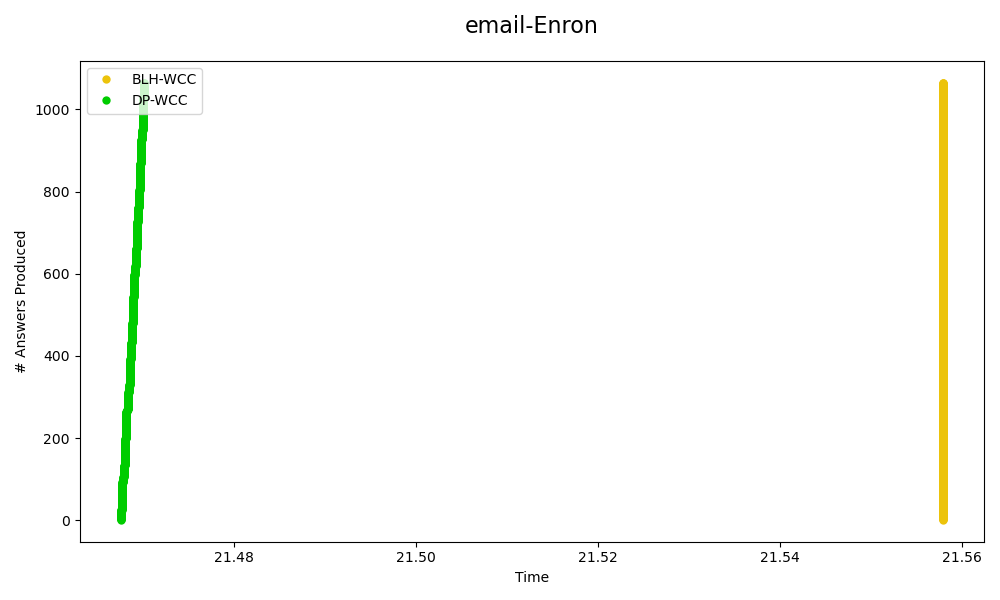
\includegraphics[width=1\linewidth, height=0.2\textheight]{email_enron0}
   \caption{email-Enron \acrlong{dm} \acrshort{dpwcc} vs. \acrshort{blwcc} Line Plot}
    \label{fig:dief:1}
  \end{subfigure}\hfill
  \begin{subfigure}[t]{0.3\textwidth}
   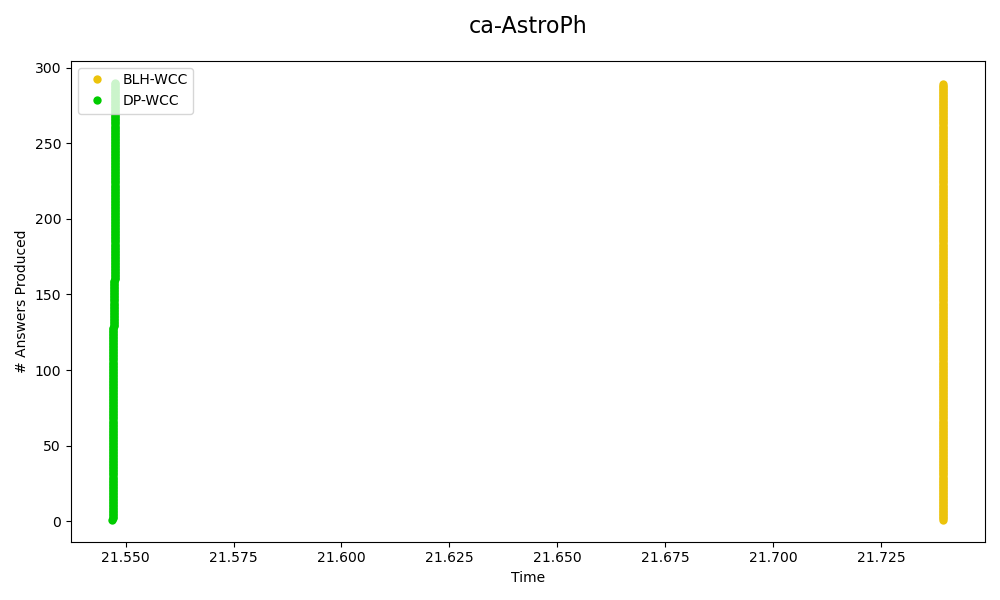
\includegraphics[width=1\linewidth, height=0.2\textheight]{ca_astroph0}
   \caption{ca-AstroPh \acrlong{dm} \acrshort{dpwcc} vs. \acrshort{blwcc} Line Plot}
    \label{fig:dief:2}
  \end{subfigure}\hfill
  \begin{subfigure}[t]{0.3\textwidth}
   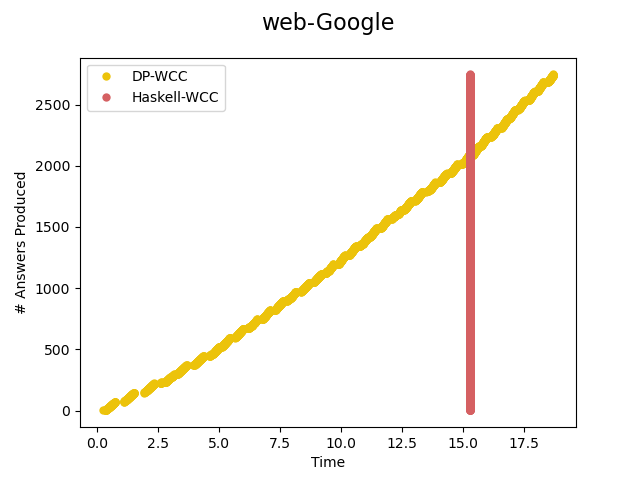
\includegraphics[width=1\linewidth, height=0.2\textheight]{web_google0}
   \caption{web-Google \acrlong{dm} \acrshort{dpwcc} vs. \acrshort{blwcc} Line Plot}
    \label{fig:dief:3}
  \end{subfigure}\hfill
   \caption{These figures show \acrshort{dt} observed results after running all the scenarios for each network with \acrshort{dpwcc} vs. \acrshort{blwcc}. $y$ axis represents the number of Answers produced and $x$ axis is the $t$ time of the \acrshort{dt} metric describe in \autoref{prem:dief}. The more data points distributed throughout the $x$ axis, the higher, the continuous behavior. The scale in axis $x$ which represents \textit{Time} is $t$, where $t$ is the microsecond difference between the start of the program and the result delivered by it.}
   \label{fig:dief:old:all}
 \end{figure}
\fi
%%%%%%%%%%%%%%%%%%%%%%%%%%%%%%%%%%%%%%%% end-Old_plots %%%%%%%%%%%%%%%%%%%%%%%%%%%%%%%%%%%%%%%%%

\begin{figure}[!htp]
  \centering
  \begin{subfigure}[t]{0.3\textwidth}
   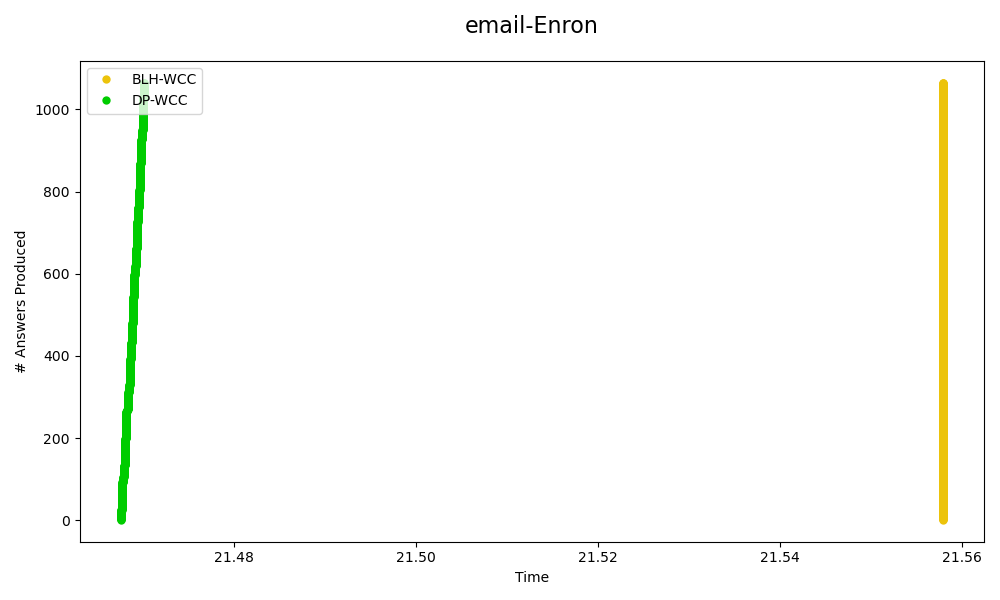
\includegraphics[width=1\linewidth, height=0.2\textheight]{email_enron0_2}
   \caption{email-Enron \acrlong{dm} \acrshort{dpwcc} vs. \acrshort{blwcc} Line Plot}
    \label{fig:dief:1}
  \end{subfigure}\hfill
  \begin{subfigure}[t]{0.3\textwidth}
   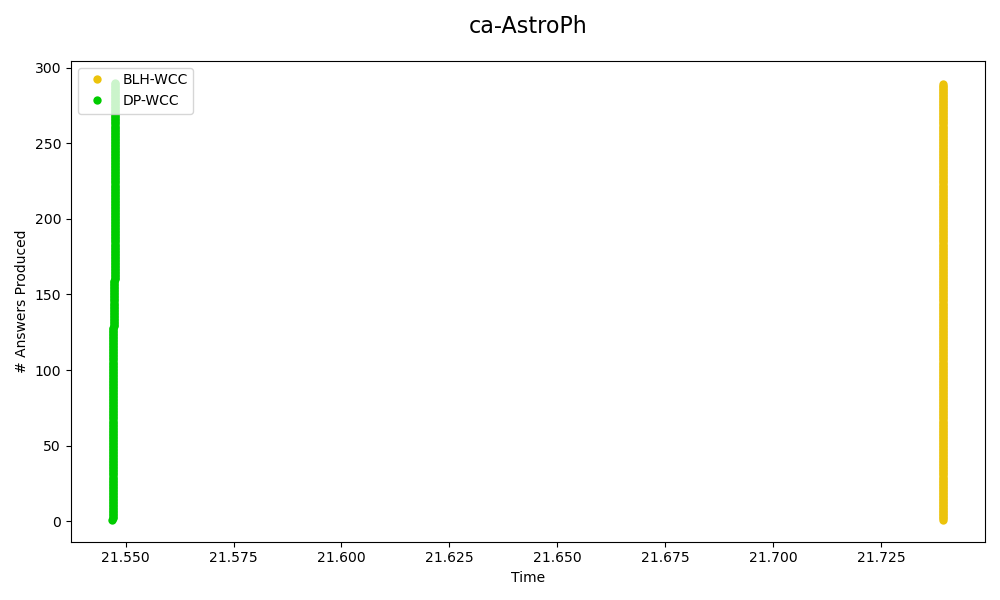
\includegraphics[width=1\linewidth, height=0.2\textheight]{ca_astroph0_2}
   \caption{ca-AstroPh \acrlong{dm} \acrshort{dpwcc} vs. \acrshort{blwcc} Line Plot}
    \label{fig:dief:2}
  \end{subfigure}\hfill
  \begin{subfigure}[t]{0.3\textwidth}
   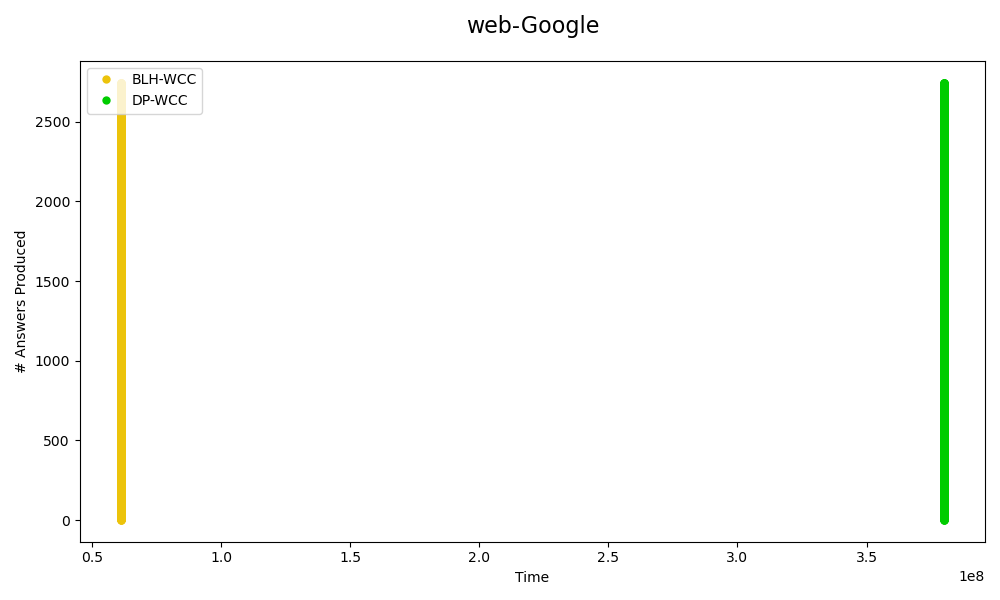
\includegraphics[width=1\linewidth, height=0.2\textheight]{web_google0_2}
   \caption{web-Google \acrlong{dm} \acrshort{dpwcc} vs. \acrshort{blwcc} Line Plot}
    \label{fig:dief:3}
  \end{subfigure}\hfill
   \caption{These figures show \acrshort{dt} observed results after running all the scenarios for each network with \acrshort{dpwcc} vs. \acrshort{blwcc}. $y$ axis represents the number of Answers produced and $x$ axis is the $t$ time of the \acrshort{dt} metric describe in \autoref{prem:dief}. The more data points distributed throughout the $x$ axis, the higher, the continuous behavior. The scale in axis $x$ which represents \textit{Time} $t$, where $t$ is the microsecond difference between the start of the program and the result delivered by it.}
   \label{fig:dief:old:all}
 \end{figure}


Based on the results shown in all the figures above, all the solutions in \acrshort{dpwcc} are being generated incrementally, but there is some difference that we would like to remark. 
In the case of \emph{email-Enron} and \emph{ca-AstroPh} graphs as we can see in \autoref{fig:dief:1} and \autoref{fig:dief:2}, there seems to be a more incremental generation of results. 
This is behavior is measured with the values of \acrfull{dt}. \emph{ca-AstroPh} as it can be seen in \autoref{fig:dief:2}, is even more incremental showing a clear separation between some results and others. 
The \emph{web-Google} network which is shown in \autoref{fig:dief:3}, is a little more linear and that is because all the results are being generated with very little difference in time between them. 
Having the biggest \acrshort{wcc} at the end of \emph{web-Google}, \acrshort{dp} algorithm it is retaining results until the biggest \acrshort{wcc} can be solved, which takes longer. 


\begin{figure}[!htp]
  \centering
  \begin{subfigure}[t]{0.3\textwidth}
   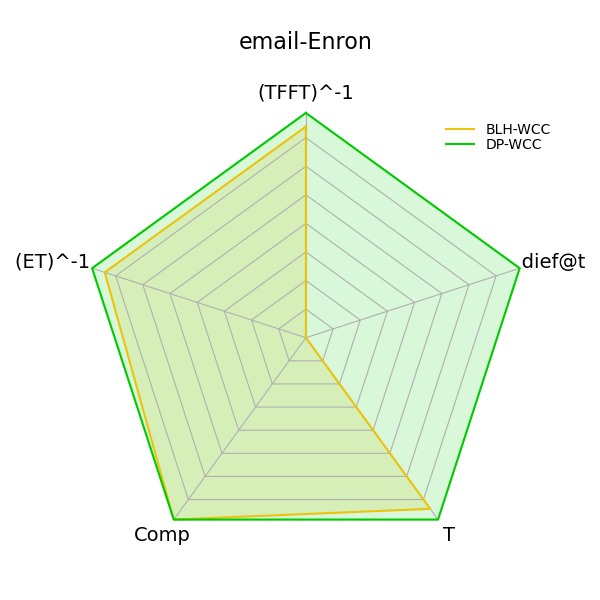
\includegraphics[width=1\linewidth, height=0.2\textheight]{email_enron_radar0_2}
   \caption{email-Enron \acrlong{dm} \acrshort{dpwcc} vs. \acrshort{blwcc} Radar Plot}
   \label{fig:dief:rad:1}
  \end{subfigure}\hfill
  \begin{subfigure}[t]{0.3\textwidth}
   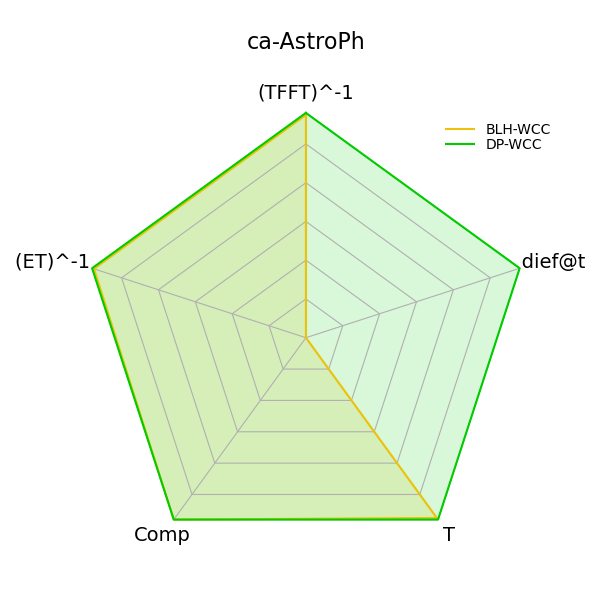
\includegraphics[width=1\linewidth, height=0.2\textheight]{ca_astroph_radar0_2}
   \caption{ca-AstroPh \acrlong{dm} \acrshort{dpwcc} vs. \acrshort{blwcc} Radar Plot}
   \label{fig:dief:rad:2}
  \end{subfigure}\hfill
  \begin{subfigure}[t]{0.3\textwidth}
   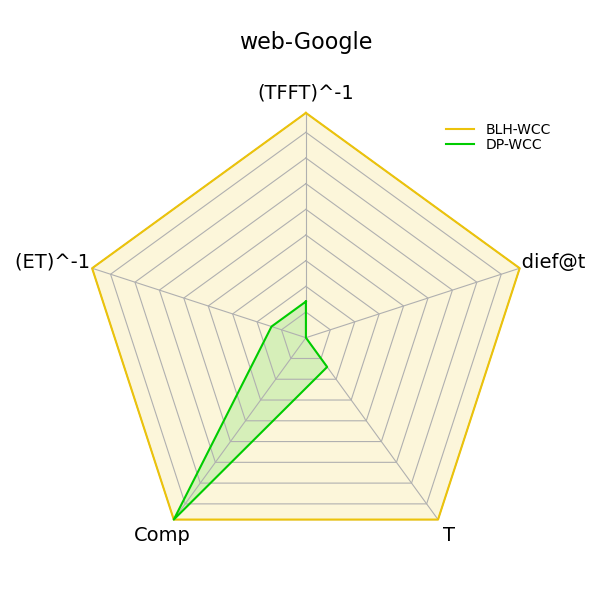
\includegraphics[width=1\linewidth, height=0.2\textheight]{web_google_radar0_2}
   \caption{web-Google \acrlong{dm} \acrshort{dpwcc} vs. \acrshort{blwcc} Radar Plot}
   \label{fig:dief:rad:3}
  \end{subfigure}\hfill
   \caption{Radial plots show how the different dimensions values provided by \acrshort{dtkp} tool such as \acrshort{tt}, \acrshort{tfft}, \acrshort{dt}, \acrshort{et} and \acrshort{comp} are related each other for each experimental case. These figures show radial plot observed results after running for each network. \acrshort{dt} is described in \autoref{prem:dief}.}
   \label{fig:dief:radial:old:all}
 \end{figure}

As we can appreciate in the above radar plots our previous analysis can be confirmed. We can see for example that the \acrlong{tt} of \emph{web-Google} in \autoref{fig:dief:rad:3}, in the case of \acrshort{dpwcc} is worse than \acrshort{blwcc}, which is not happening for the others.
We can say that regarding [Q2] (\autoref{res:question}) although \acrshort{dpwcc} is faster than the traditional approach, the speed-up dimension execution factor is not always the most interest analysis that we can have, because as we have seen even when in the case of \emph{web-Google} Graph \acrshort{dpwcc} is slower at execution, it is at least generating incremental results without the need to wait for the rest of the computations.

Moreover, we have run a comparison analysis between \acrshort{dpwcc} and \acrshort{dpfhwcc}, using the same \acrlong{dm}, to confirm the new implementation \acrshort{dpfhwcc} is still presenting continuous behavior delivering incremental results.

\begin{table}[htp!]
  \centering
  \begin{tabular}{|p{0.25\linewidth}|c|c|c|}
    \hline
   \textbf{Network} & \textbf{Implementation} & \textbf{dief@t Metric}  & \textbf{dief@k Metric}\\
   \hline
   \multirow{2}{*}{ca-AstroPh} & \acrshort{dpfhwcc} & $1.27 \times 10^8$ & $1.80 \times 10^5$\\
   & \acrshort{dpwcc} & $8.77 \times 10^5$ & $8.77 \times 10^5$\\
   \hline
   \multirow{2}{*}{email-Enron} & \acrshort{dpfhwcc} & $7.42 \times 10^8$ & $1.38 \times 10^6$\\
   & \acrshort{dpwcc} & $1.98 \times 10^6$ & $1.98 \times 10^6$\\
   \hline
   \multirow{2}{*}{web-Google} & \acrshort{dpfhwcc} & $1.29 \times 10^7$ & $1.29 \times 10^7$ \\
   & \acrshort{dpwcc} & $2.35 \times 10^{10}$ & $1.17 \times 10^7$\\
  \hline
  \end{tabular}
  \caption{This tables shows the \acrshort{dt} and \acrshort{dk} values gather for  $\dpwcc$ in \acrshort{dpfh}. We can appreciate that in all cases $\dpwcc$ has a higher value of \acrshort{dt} and a lower value of \acrshort{dk} showing continuos behavior}
 \label{table:e1:dm:values}
 \end{table}

\begin{figure}[!htp]
  \centering
  \begin{subfigure}[t]{0.3\textwidth}
   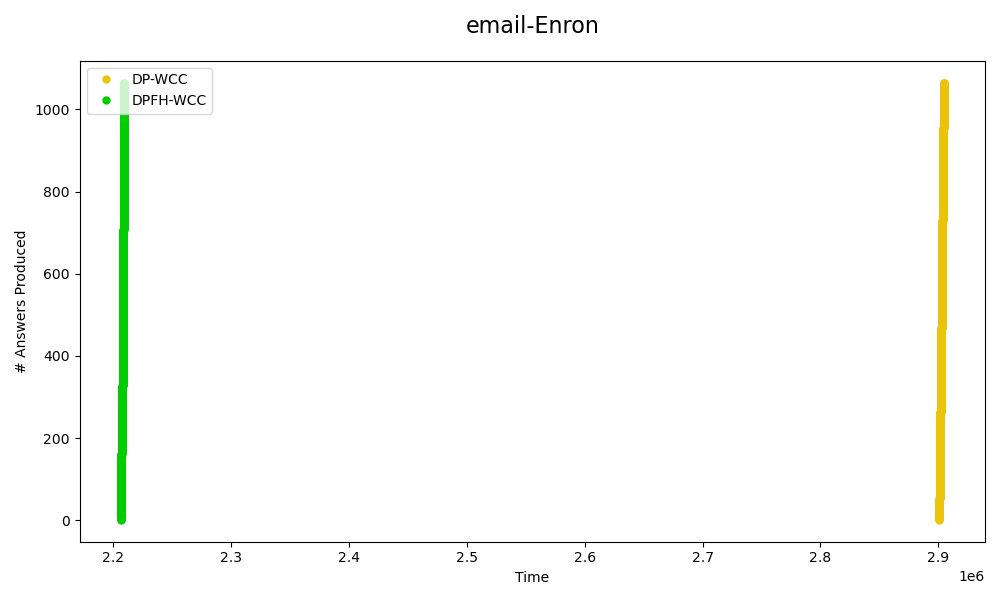
\includegraphics[width=1\linewidth, height=0.2\textheight]{email_enron}
   \caption{email-Enron \acrlong{dm} \acrshort{dpfhwcc} vs. \acrshort{dpwcc} Line Plot}
    \label{fig:dief:new:1}
  \end{subfigure}\hfill
  \begin{subfigure}[t]{0.3\textwidth}
   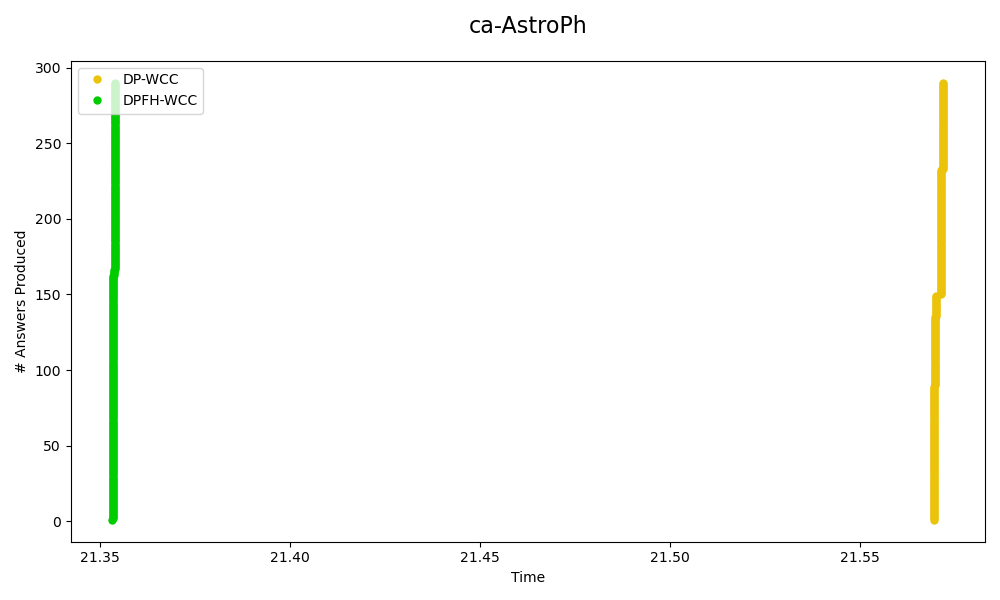
\includegraphics[width=1\linewidth, height=0.2\textheight]{ca_astroph}
   \caption{ca-AstroPh \acrlong{dm} \acrshort{dpfhwcc} vs. \acrshort{dpwcc} Line Plot}
    \label{fig:dief:new:2}
  \end{subfigure}\hfill
  \begin{subfigure}[t]{0.3\textwidth}
   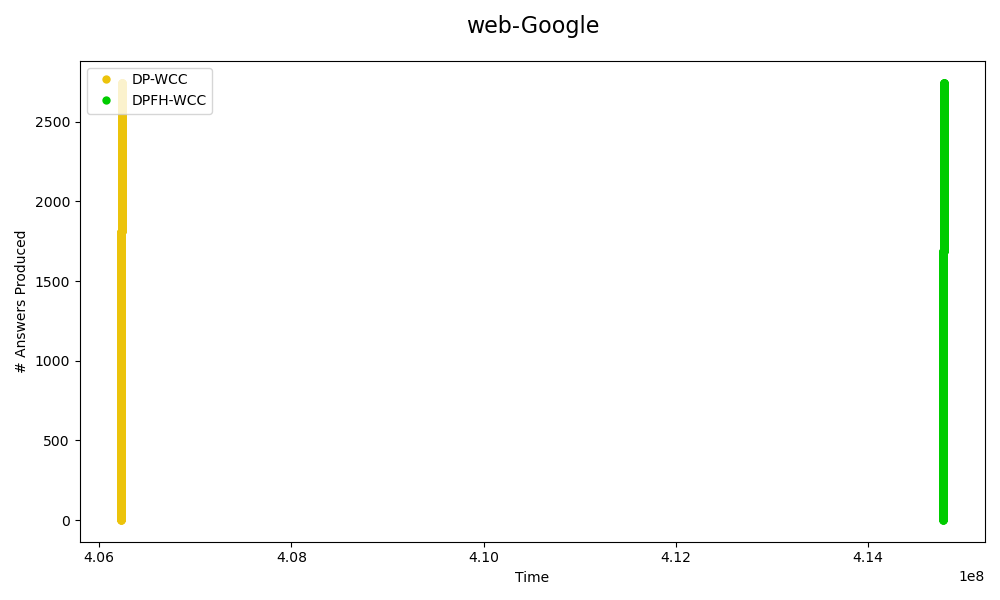
\includegraphics[width=1\linewidth, height=0.2\textheight]{web_google}
   \caption{web-Google \acrlong{dm} \acrshort{dpfhwcc} vs. \acrshort{dpwcc} Line Plot}
    \label{fig:dief:new:3}
  \end{subfigure}\hfill
   \caption{These figures show \acrshort{dt} observed results after running all the scenarios for each network with \acrshort{dpfhwcc} vs. \acrshort{dpwcc}. $y$ axis represents the number of Answers produced and $x$ axis is the $t$ time of the \acrshort{dt} metric describe in \autoref{prem:dief}. The more data points distributed throughout the $x$ axis, the higher, the continuous behavior. The scale in axis $x$ which represents \textit{Time} $t$, where $t$ is the microsecond difference between the start of the program and the result delivered by it.}
   \label{fig:dief:all}
 \end{figure}


 \begin{figure}[!htp]
  \centering
  \begin{subfigure}[t]{0.3\textwidth}
   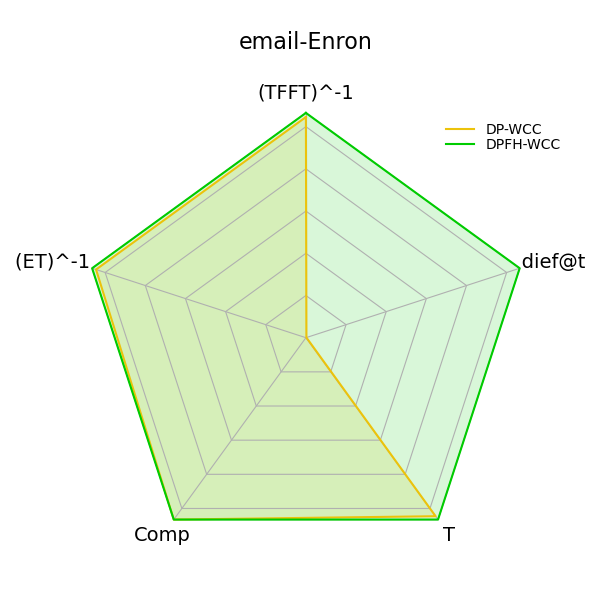
\includegraphics[width=1\linewidth, height=0.2\textheight]{email_enron_radar}
   \caption{email-Enron \acrlong{dm} \acrshort{dpfhwcc} vs. \acrshort{dpwcc} Radar Plot}
    \label{fig:dief:rad:new:1}
  \end{subfigure}\hfill
  \begin{subfigure}[t]{0.3\textwidth}
   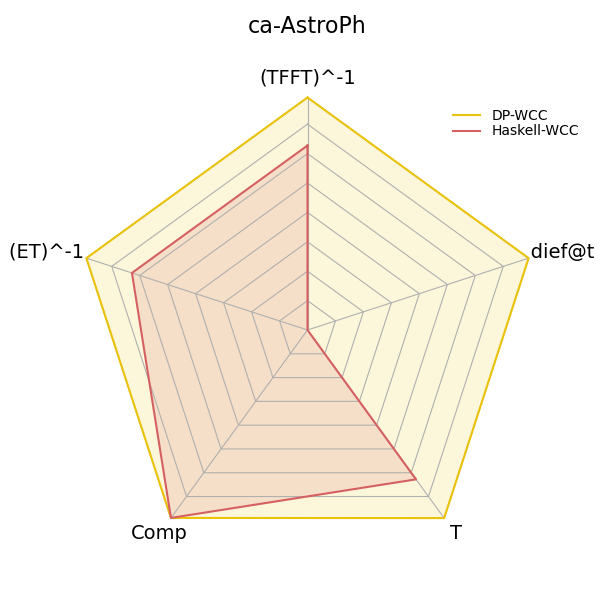
\includegraphics[width=1\linewidth, height=0.2\textheight]{ca_astroph_radar}
   \caption{ca-AstroPh \acrlong{dm} \acrshort{dpfhwcc} vs. \acrshort{dpwcc} Radar Plot}
    \label{fig:dief:rad:new:2}
  \end{subfigure}\hfill
  \begin{subfigure}[t]{0.3\textwidth}
   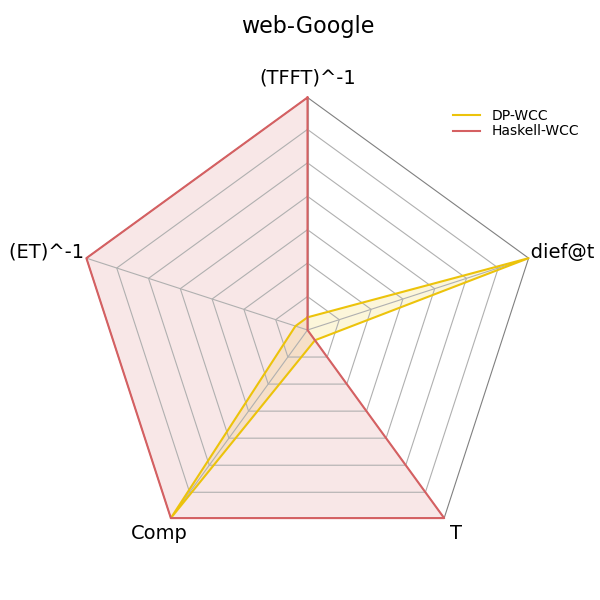
\includegraphics[width=1\linewidth, height=0.2\textheight]{web_google_radar}
   \caption{web-Google \acrlong{dm} \acrshort{dpfhwcc} vs. \acrshort{dpwcc} Radar Plot}
    \label{fig:dief:rad:new:3}
  \end{subfigure}\hfill
   \caption{Radial plots show how the different dimensions values provided by \acrshort{dtkp} tool such as \acrshort{tt}, \acrshort{tfft}, \acrshort{dt}, \acrshort{et} and \acrshort{comp} are related each other for each experimental case. These figures show radial plot observed results after running for each network. \acrshort{dt} is described in \autoref{prem:dief}.}
   \label{fig:dief:radial:all}
 \end{figure}

Based on the results shown in \autoref{fig:dief:all} and with the support of the metrics values in \autoref{table:e1:dm:values}, it can be appreciated that both solutions, \acrshort{dpwcc} and \acrshort{dpfhwcc} show continuous behavior.
Moreover, in \autoref{table:e1:dm:values}, \acrshort{dpfhwcc} has a higher value of \acrshort{dt} and a lower value of \acrshort{dk} for \textit{ca-AstroPh} and \textit{email-Enron} confirming the continuous behavior. In the case of \textit{web-Google} which is the biggest network, \acrshort{dpwcc} seems to be more continuous than \acrshort{dpfhwcc} according to its \acrshort{dt} and \acrshort{dk} values, but that does not mean that \acrshort{dpfhwcc} is not continuous. If that was the case its values should be $0$.
As we can appreciate in \autoref{fig:dief:radial:all} radar plots also confirm our previous analysis on continuity.

In conclusion, we can say that regarding [RQ2] (\autoref{res:question}) although \acrshort{dpwcc} is faster and more continuous in \emph{web-Google} Graph, \acrshort{dpfhwcc} is much more faster and more continuous in the other networks, showing that it enhance the continuity approach.

\paragraph{Experiment: E3}
For this type of analysis, our experiment focuses on \emph{email-Enron} network  only because profiling data generated by \acrshort{ghc} is big enough to conduct the analysis and on the other, and enabling profiling penalize execution time.
Moreover, it is important to remark that the analysis was conducted on \acrshort{dpwcc} and \acrshort{dpfhwcc} but since the results are similar in terms of plots and behavior, we show only the results obtained for \acrshort{dpwcc} measurements.

\paragraph{Multithreading} For analyzing parallelization and multithreading we have used \textit{ThreadScope} Tool  which allows us to see how the parallelization is taking place on \acrshort{ghc} at a fine grained level and how the threads are distributed throughout the different cores requested with the \mintinline{bash}{-N} execution \texttt{ghc-option} flag.

\begin{minipage}[t!]{\linewidth}

  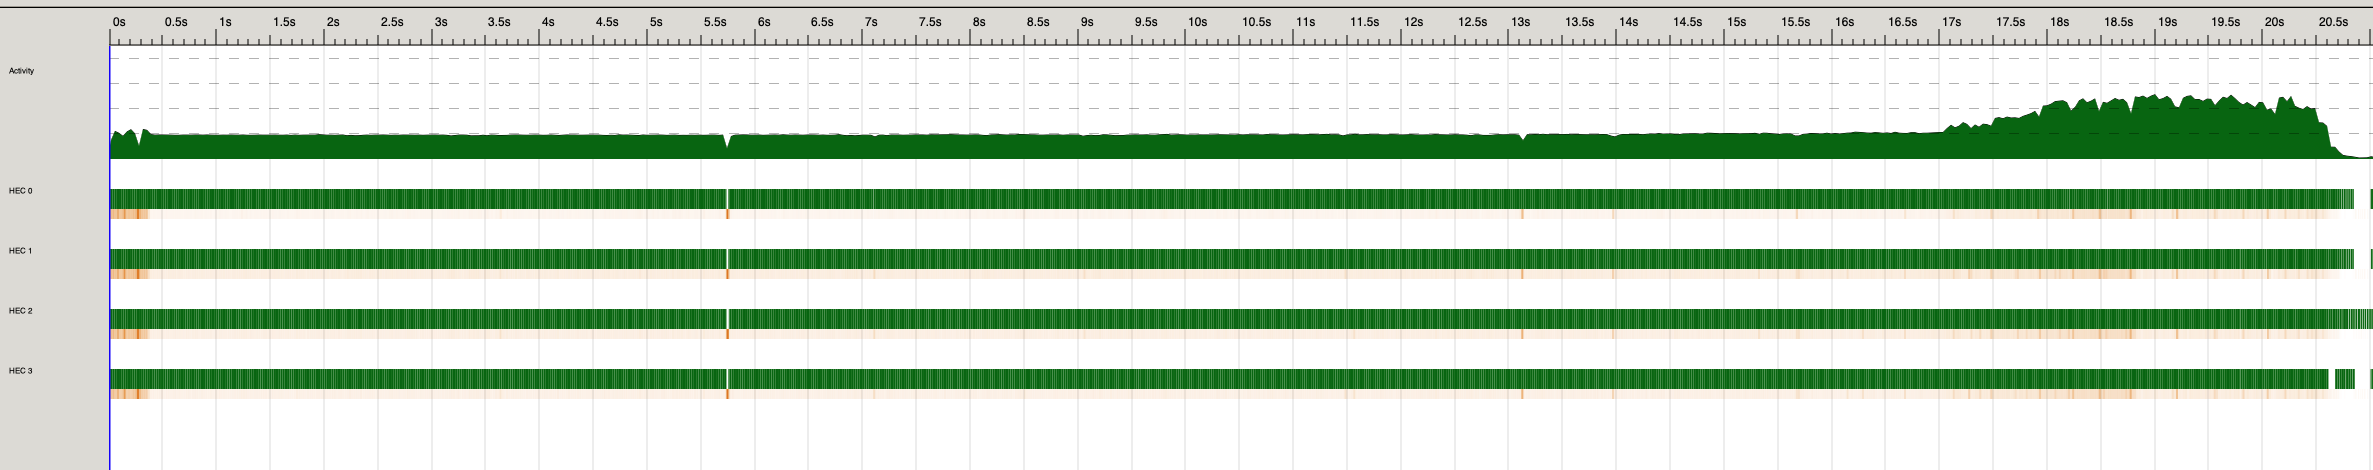
\includegraphics[width=\textwidth]{screen_1}
  \captionsetup{type=figure}
  \captionof{figure}{Threadscope Image of General Execution}
  \label{fig:3}
\end{minipage}

In \autoref{fig:3}, we can see that the parallelization is being distributed evenly among the $4$ Cores that we have set for this execution.
The distribution of the load is more intensive at the end of the execution, where \mintinline{haskell}{actor2} filter stage 
%as it can be seen in \autoref{src:haskell:3}, 
of the algorithm is taking place and different filters are reaching execution of that second actor.

\begin{wrapfigure}{r}{0.5\textwidth}
  \begin{center}
     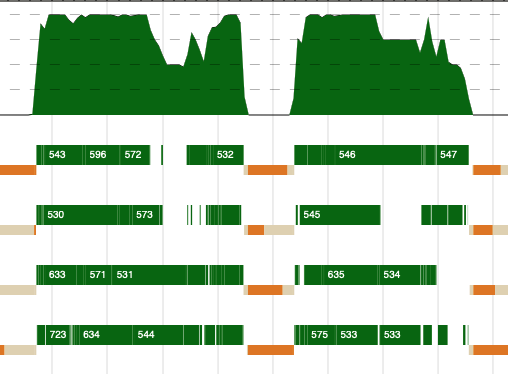
\includegraphics[width=0.48\textwidth] {screen_2}
     %[width=10cm, height=9cm]
       \end{center}
     \caption{Threadscope Image of Zoomed Fraction}
     \label{fig:4}
 %\end{figure}
 \end{wrapfigure}
Another important aspect shown in \autoref{fig:3}, is that this work is not so significant for \acrshort{ghc} and the threads and distribution of the work keeps between 1 or 2 cores during the execution time of the \mintinline{haskell}{actor1}. However, the usages increase on the second actor as pointed out before. In this regard, we can answer research questions [Q1] and [Q3] (\autoref{res:question}), verifying that \acrshort{hs} not only supports the required parallelization level but is evenly distributed across the program execution too.

Finally, it can also be appreciated that there is no sequential execution on any part of the program because the $4$ cores have \textit{CPU} activity during the whole execution time. This is because as long the program start, and because of the nature of the \acrshort{dp} model, it is spawning the \textit{Source} stage in a separated thread. This is a clear advantage for the model and the processing of the data since the program does not need to wait to do some sequential processing like reading a file, before start computing the rest of the stages.




%\begin{minipage}[t!]{\linewidth}
%\begin{center}
%  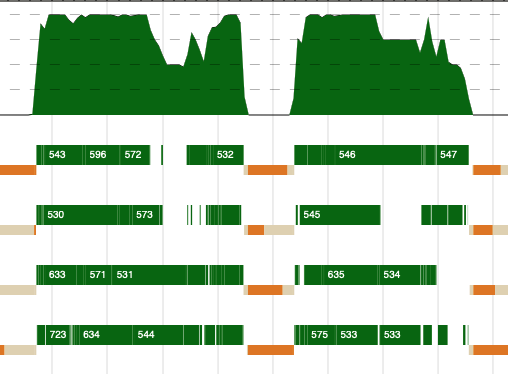
\includegraphics[width=0.6\textwidth]{screen_2}
%  \captionsetup{type=figure}
%  \captionof{figure}{Threadscope Image of Zoomed Fraction}
%  \label{fig:4}
%  \end{center}
%\end{minipage}

\autoref{fig:4} zooms in on \textit{ThreadScope} output in a particular moment, approximately in the middle of the execution. We can appreciate how many threads are being spawned and by the tool and if they are evenly distributed among cores. The numbers inside green bars represent the number of threads that are being executed on that particular core (horizontal line) at that execution slot. Thus, the number of threads varies among slot execution times because, as it is already known, \acrshort{ghc} implements \emph{Preemptive Scheduling} \cite{lightweightghc}.

Having said that, it can be appreciated in \autoref{fig:4} our first assumption that the load is evenly distributed because the mean number of executing threads per core is $571$.

\paragraph{Memory allocation} Another important aspect in our case is how the memory is being managed to avoid memory leaks or other non-desired behavior that increases memory allocation during the execution time. This is even more important in the particular implementation of \acrshort{wcc} using \acrshort{dp} model because it requires to maintain the set of connected components in memory throughout the execution of the program or at least until we can output the calculated \acrshort{wcc} if we reach to the last \textit{Filter} and we know that this \acrshort{wcc} cannot be enlarged anymore. 

In order to verify this, we measure memory allocation with \textit{eventlog2html} which converts generated profiling memory eventlog files into graphical HTML representation. 

\begin{wrapfigure}{r}{0.5\textwidth}
  \begin{center}
     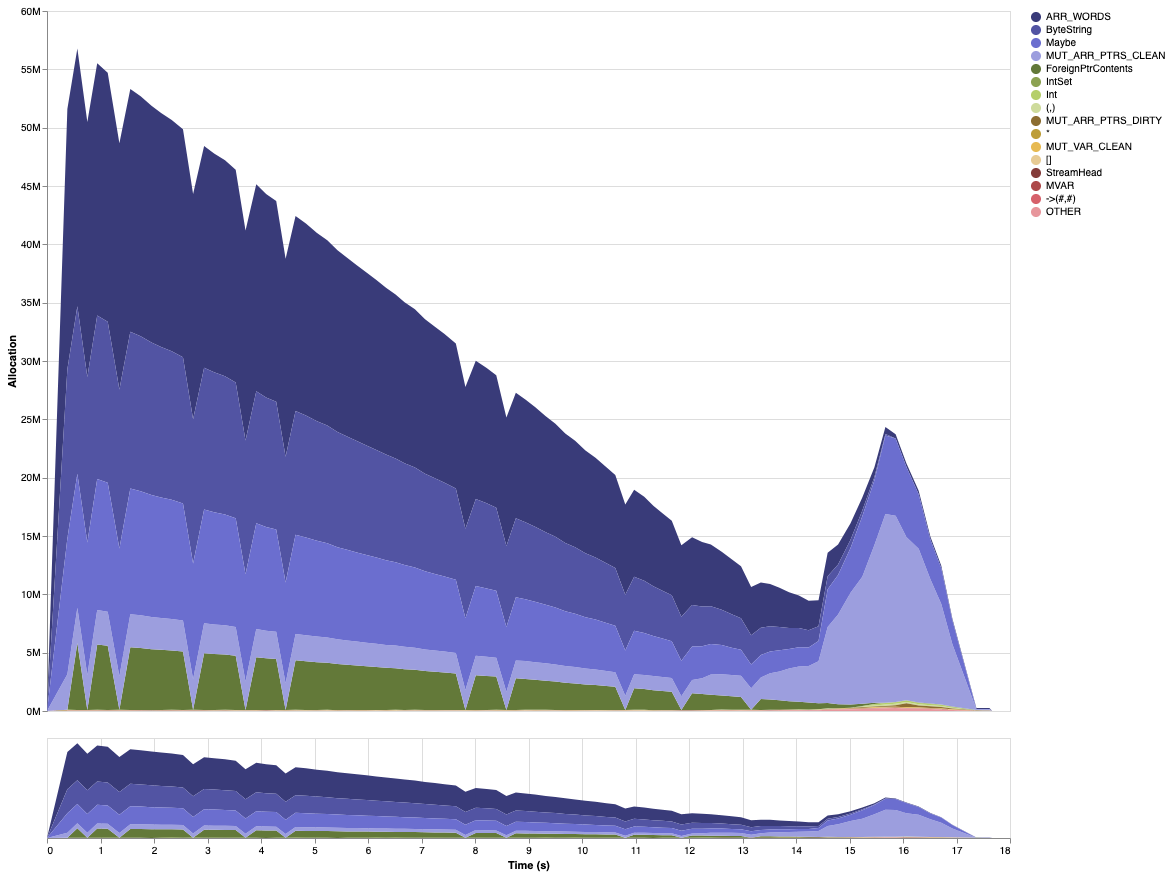
\includegraphics[width=0.5\textwidth] {visualization}
     %[width=10cm, height=9cm]
       \end{center}
     \caption{Memory Allocation}
     \label{fig:5}
 %\end{figure}
 \end{wrapfigure}
 
%\begin{minipage}[t]{\linewidth}
%\begin{center}
%  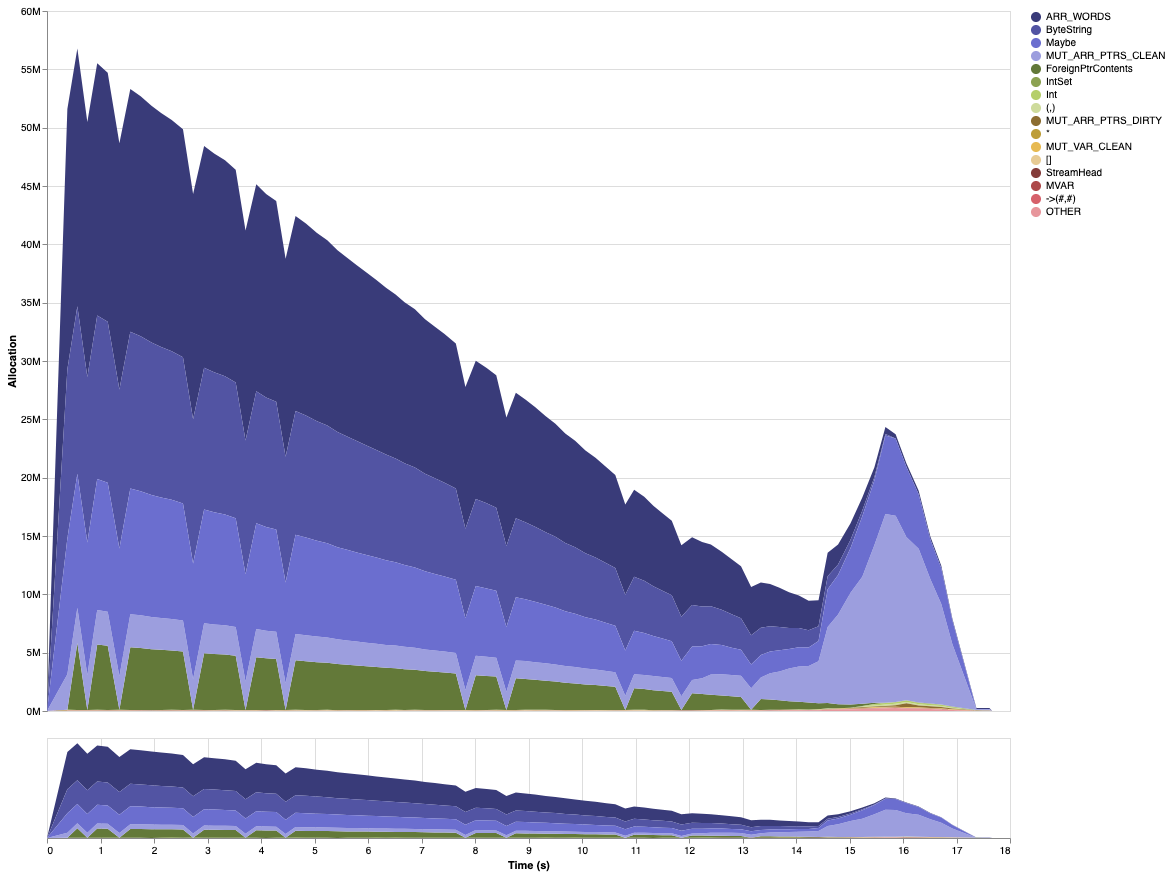
\includegraphics[width=0.6\textwidth]{visualization}
%  \captionsetup{type=figure}
%  \captionof{figure}{Memory Allocation}
%  \label{fig:5}
%  \end{center}
%\end{minipage}

As we can see in \autoref{fig:5}, \acrshort{dpwcc} does an efficient work on allocating memory since we are not using more than $57$ MB of memory during the whole execution of the program.

On the other hand, if we analyze how the memory is allocated during the execution of the program, it can also be appreciated that most of the memory is allocated at the beginning of the program and steadily decrease over time with a small peak at the end that does not overpass even half of the initial peak of $57$ MB. The explanation for this behavior is quite straightforward because at the beginning we are reading from the file and transforming a \mintinline{haskell}{ByteString} buffer to \mintinline{haskell}{(Int, Int)} edges. This is seen in the image in which the dark blue that is on top of the area is \mintinline{haskell}{ByteString} allocation. Light blue is allocation of \mintinline{haskell}{Maybe a} type which is the type that is returned by the \textit{Channels} because it can contain a value or not. Data value \mintinline{haskell}{Nothing} is indicating end of the \textit{Channel}.  
%as we can see in \autoref{src:haskell:f3}.

Another important aspect is the green area which represents \mintinline{haskell}{IntSet} allocation, which in the case of our program is the data structure that we use to gather the set of vertices that represents a \acrshort{wcc}. This means that the amount of memory used for gathering the \acrshort{wcc} itself is minimum, and it is decreasing over time, which is another empirical indication that we are incrementally releasing results to the user. It can be seen as well that as long the green area reduces the lighter blue (\mintinline{haskell}{MUT_ARR_PTRS_CLEAN}\footnote{\href{https://downloads.haskell.org/~ghc/8.10.4/docs/html/libraries/ghc-heap-8.10.4/GHC-Exts-Heap-ClosureTypes.html}{GHC-Exts-Heap-ClosureTypes.html}}) increases at the same time indicating that the computations for the output (releasing results) is taking place. 

Finally, according to what we have stated above, we can answer the question [Q3] (\autoref{res:question}) showing that not only memory management was efficient, but at the same time, the memory was not leaking or increasing across the running execution program.

The empirical evaluation of \acrshort{dpwcc} evidences suitability, and robustness of this language to of  support the development of a Dynamic Pipeline Framework. Measuring using diefficienc metrics reveals some advantageous capability of $\dpwcc$ implementation to deliver incremental results compared with default containers library implementation.  Regarding the main aspects where DPP is strong, i.e., pipeline parallelism and time processing, the $\dpwcc$ performance shows that Haskell can deal with the requirements for the \acrshort{wcc} problem without penalizing neither execution time nor memory allocation. In particular, the $\dpwcc$ implementation outperforms in those cases where the topology of the graph is sparse and where the number of vertices in the largest \acrshort{wcc} is not big enough.  

To conclude, \acrshort{dpwcc} has gathered enough evidence to show that the implementation of a Dynamic Pipeline solutions in Haskell Programming Language is feasible. This fact opens a wide range of algorithms to be explored using the Dynamic Pipeline Paradigm, supported by purely functional programming language. This results give us insights about how to proceed for implementing a first version of a DPF using (parallel) Haskell.